
\chapter{Acoustic Observations in Event 50}



Our goal in SW06 experiment is specifically to examine the relationship between internal wave and acoustic wave propagation. In particular we seek to understand the acoustic wave propagation mechanisms governed by the direction of the acoustic track relation to the internal wave front. 


The propagation of acoustic signals is strongly related to the ocean's physical attributes with various time scales and frequencies, such as surface waves, internal waves, tides, currents. Given the conditions of SW06 experiment  ( acoustic signal transmission interval = 4sec, acoustic listening window = 3hr), we concentrated ourselves to the variation caused by the internal wave activities. 

Quantities will be used in the following sections are:

\begin{enumerate}


\item Integrated acoustic intensity  

When the propagation and scattering conditions change in the water, the received acoustic intensity changes at the same time. We calculate the intensity of the signal arrivals integrated over a pulse
length $\Delta\tau$ at a given depth $z$ as

\begin{equation}\label{eq:intensity1}
I(z,T)=\displaystyle\frac{1}{{\rho}c}\int\limits^{\tau+\Delta\tau}_{\tau}p^2(z,T,t)\,dt
\end{equation}
where $p$ is acoustic
pressure,$\rho$ is water density, and $c$ is sound speed.
And the total intensity integrated over the depth H is

\begin{equation}\label{eq:intensity2}
I(T)=\displaystyle\int\limits^H_0I(z,T)dz.
\end{equation}
The time integration at a single hydrophone is to show the attenuation and scattering through the medium, both horizontally and vertically, thus carries much information about the environment, in our case the internal wave packet. On the other hand, the depth integration over the entire water column gives the energy flux through a particular vertical slice, which is of great interests here because the change of this parameter shows how much energy is transported through the horizontal acoustic mechanisms like refraction and reflection, under the condition of constant attenuation and scattering. 
We will examine the mean and standard deviations of the intensity at different stages during the passing of the internal wave packet. 

\item arrival time and pulse spread

The passing of the internal waves also has an effect at the arrival time (sometimes called the "wander" in literature) and pulse spread. We define the arrival time as the arrival time of the centroid of the acoustic pulse.
\begin{equation}\label{eq:arrival_time}
t_c =\frac {\int\limits^{t_0}_{t_1}I(t)tdt}{\int\limits^{t_0}_{t_1}I(t)dt}
\end{equation} 
in which, $t_c$ is the arrival time, $t_0$ and $t_1$ are the beginning and the end time of a received pulse, $I(t)$ is the acoustic intensity. (All the time variables in the equation above $t_c$,$t_0$,$t_1$ are started from a common but arbitrary zero point, due to the lack of a absolute clock between the receiver and the transmitter. )
There are other definitions of the "arrival time" in the literature, e.g. the leading edge arrival time and the peak arrival time. We choose the centroid definition due to its insensitivity to the swift changes of the arrival pulse structure, which are quite common in SW06 experiment. 

The pulse spread is the duration of the acoustic pulse after matched filter. We consider the received acoustic signal is part of the pulse, if its level is 10 times bigger than the mean noise level, which is measured during the quiet time between transmissions.

\end{enumerate}
%\begin{figure}[H]
%  \centering
%  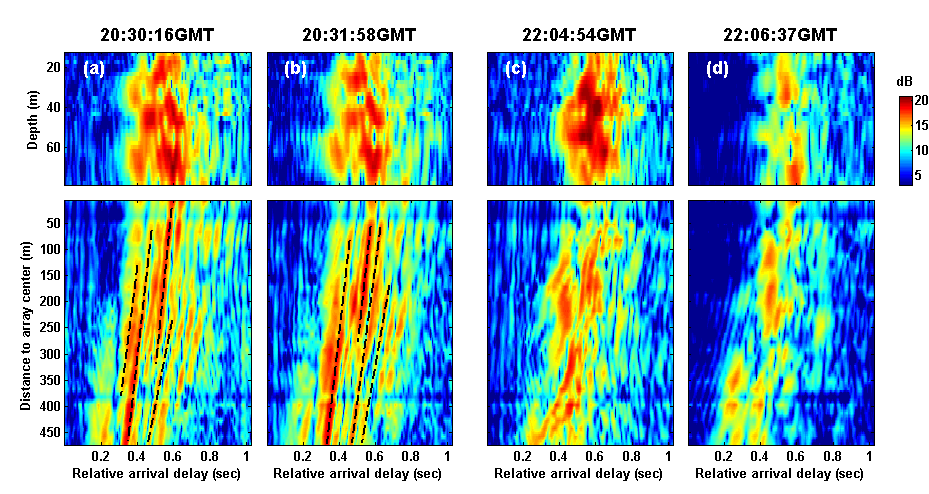
\includegraphics[width=0.75\textwidth]{jasa3.png}
%  \caption{Received acoustic intensity on the Shark VHLA during two geotimes within the $T_{g1}$ and $T_{g2}$ periods. Upper panel shows the acoustic field on the VLA portion of the array while the lower panel shows the HLA portion. (a) Tg = 20:30:16 GMT, (b) Tg = 20:31:58 GMT, (c) Tg = 22:04:54 GMT, (d) Tg = 22:06:37 GMT.}\label{fig:jasa3}
%\end{figure}
%
%Next, we show the acoustic signal arrival on the Shark VHLA during
%the two periods $T_{g1}$ and $T_{g2}$. In order to show the intensity
%variations, we show the arrival of two different LFM pings on the
%array at geotimes separated by 102 sec. In Fig.\ref{fig:jasa3}, the upper
%panel shows the acoustic signal on the VLA at 20:30:16 GMT while the
%lower panel shows the same signal arriving on the HLA. Figure 3(b)
%shows the same two arrays at 20:31:58 GMT. The parallel lines on the
%HLA data shown in the lower panels are due to the difference of
%arrival time on the HLA (see array configuration in Fig. 1(c)). The
%data on the VLA portion of the array shown in the upper panels best
%represent the modal arrivals. Note the similarity of the intensity
%values on both vertical and the horizontal array plots in Figs. 3(a)
%and 3(b), indicating the stability of the arriving signal energy
%during $Tg_1$. During $Tg_2$ the same data format is shown. At
%22:04:54 GMT shown in Fig. 3(c), both the VLA and HLA show a drastic
%change in the arrival. The signal intensity becomes very strong;
%however, different  arrivals are mixed together and difficult to
%separate. The parallel lines on the HLA were notably distorted. At
%22:06:37 GMT shown in Fig. 3(d), the arrivals show a lack of
%structure as well as lower intensity. During the time period of $T_{g2}$,
%the ISW is occupying a large fraction of the acoustic track. Mm. 2
%shows a movie of the acoustic signal arrival on the Shark VHLA
%during the two periods $T_{g1}$ and $T_{g2}$. To further quantify these
%results, we next calculate the average intensity in geotime and
%depth for the periods, $Tg_1$ and $Tg_2$.
%
%Figure \ref{fig:zones} showing the positions of the acoustic sources. (a) NRL 300Hz source was fixed at lat. $39.18^o$ long. $72.94^o$ and transmitted 7 minutes of data every half hour, (b) J15 source was deployed below R/V Sharp positioned at the front of IW Rosey (Event 50) follow the propagation of the IW. This source transmitted signals fro 15 minutes every half hour and was quite during the time when NRL source was on. This way it was assured that there were continuous transmission during the IW passage. In addition, the R/V Sharp source provided acoustic source hanging below the ship at fixed position with respect to R/V Sharp which was moving with the front of IW (at ~0.5m/s) and transmitted during the quiet periods when NRL source was down.

\section{Transmission from the fixed source(NRL 300Hz)}

This part of the experiment can be roughly divided into four phases based on the distance between the acoustic path and the IW packet.

\subsection{Phase I: 20:30-20:37GMT \& 21:00-21:07GMT}
Phase I is the quiescent time before the internal wave packet arrive at the source-receiver track and have little impact on the acoustic propagation.  
Figure \ref{fig:r2030_i} show the interpolated radar images at the beginning of the transmissions (20:30GMT). The leading front of the IW packet is at about 6 kilometers away at the closest point (SHARK VLA) of the acoustic track. Integrated intensity of the received signals ( squared matched filter output) on Shark VHLA are plotted in Fig. \ref{fig:a2030} for the transmission from 20:30 through 20:37GMT, where, the top and bottom panel shows the received signal on VLA and HLA and the middle palel shows the depth integrated signal intensity. The VLA panel shows a stable 3-stripe pattern, which can be attributed to the strong 2nd and 3rd modes (Fig. \ref{fig:m2030}). The acoustic energy has a clear concentration at the lower part of the receiver array,  below the thermocline (~15m from the surface). The fluctuation of the depth integrated intensity is less than 2.5dB. The results of the next transmission (21:00-21:07GMT) are similar to what we observed here ( Fig. \ref{fig:r2100_i}, \ref{fig:a2100} and \ref{fig:m2100}). The signals received during these two transmission help us establish the base scenarios to compare with the acoustic propagation in the later phases.
%
% which, after modal decomposition (Fig.\ref{fig:m2030}), can be
%attributed to the strong and steady 2nd and 3rd modes. 
%Although the fluctuation of the total
%intensity is less than 2.5dB, from the modal amplitude plot, we can
%see the increase of the intensity mode 1 and 4 and the decrease of
%mode 2 and 3. The energy exchange among the different modes here
%suggest the occurrence of the modal coupling.


%\begin{figure}[H]
 % \centering
  %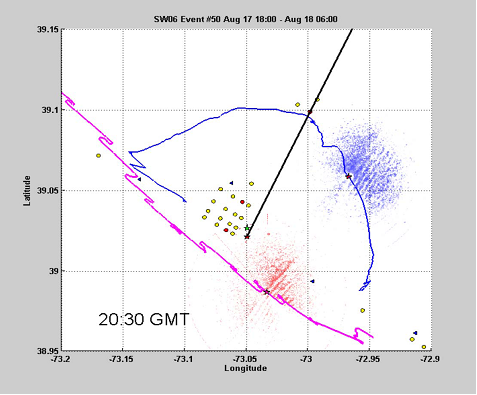
\includegraphics[width=0.5\textwidth]{radar2030.png}
  %\caption{Radar image of ISW at 20:30GMT}\label{fig:r2030}
%\end{figure}
%
%\begin{figure}
%  \centering
%  \begin{tabular}{l}
%  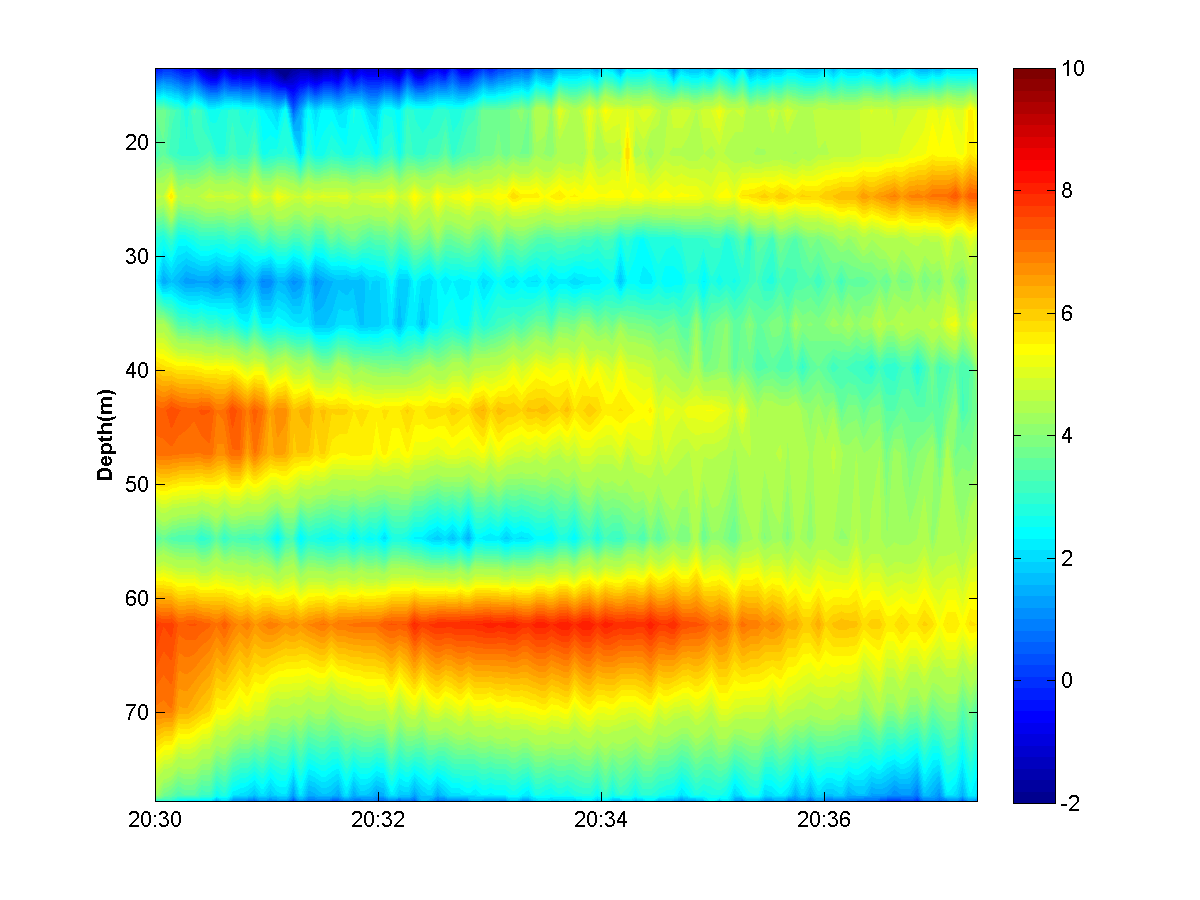
\includegraphics[width=0.5\textwidth,height=0.2\textwidth]{0817_2030_vla.png}\\
%  \ 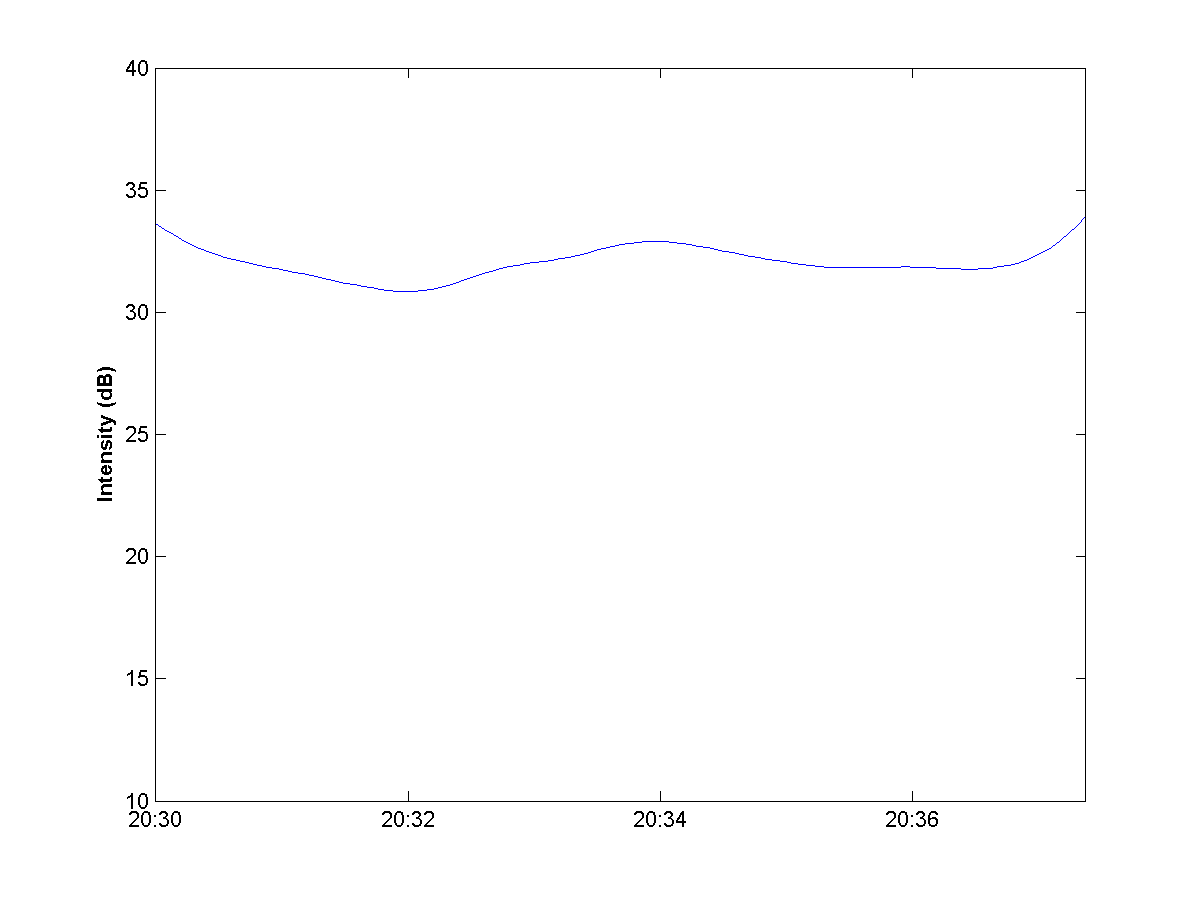
\includegraphics[width=0.44\textwidth,height=0.2\textwidth]{0817_2030_eng.png}\\
%  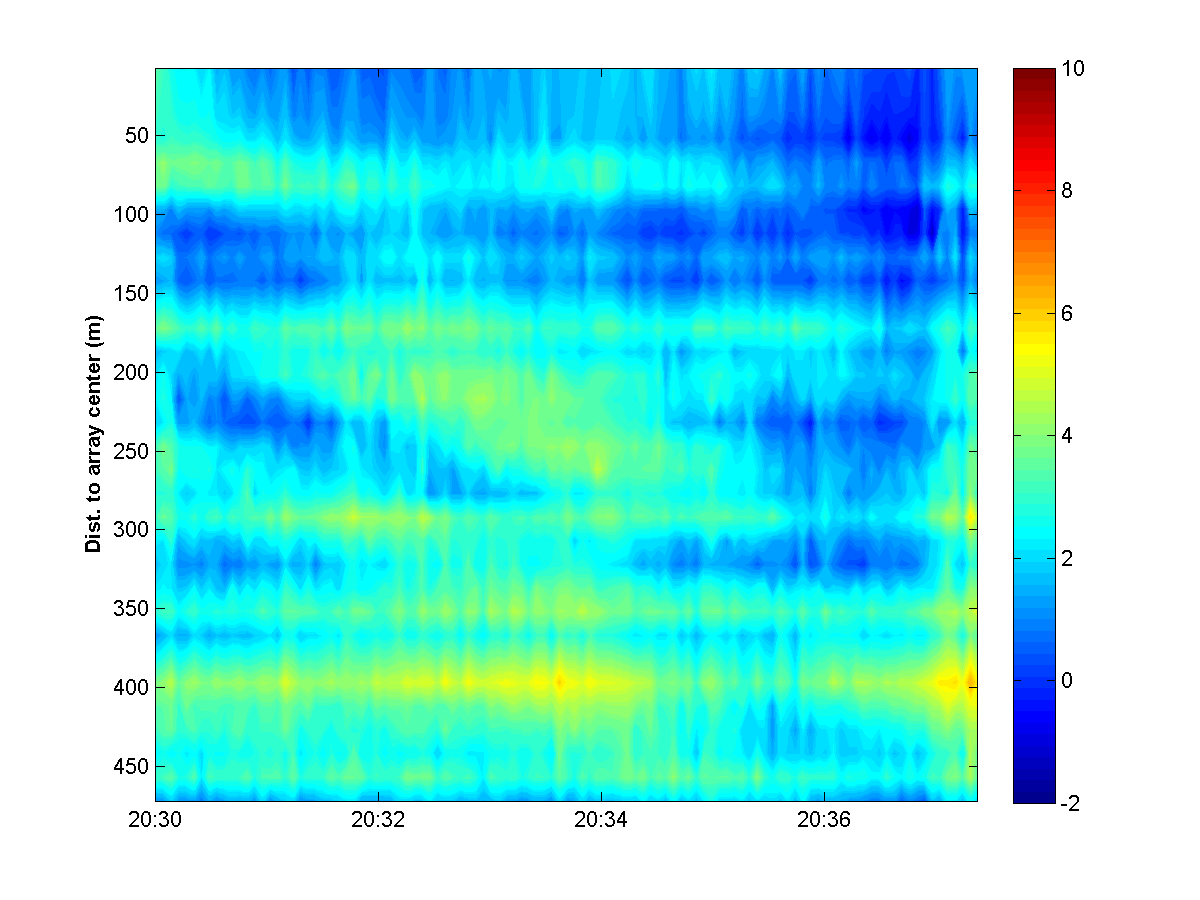
\includegraphics[width=0.5\textwidth,height=0.2\textwidth]{0817_2030_hla.png}\\
%  \end{tabular}
%  \caption{Received signal on Shark VLA (top), HLA (bottom) and signal intensity (middle) from Aug.17 20:30GMT to 20:37GMT }\label{fig:a2030}
%\end{figure}

%\begin{figure}
 % \centering
 % \begin{tabular}{lrr}
 % 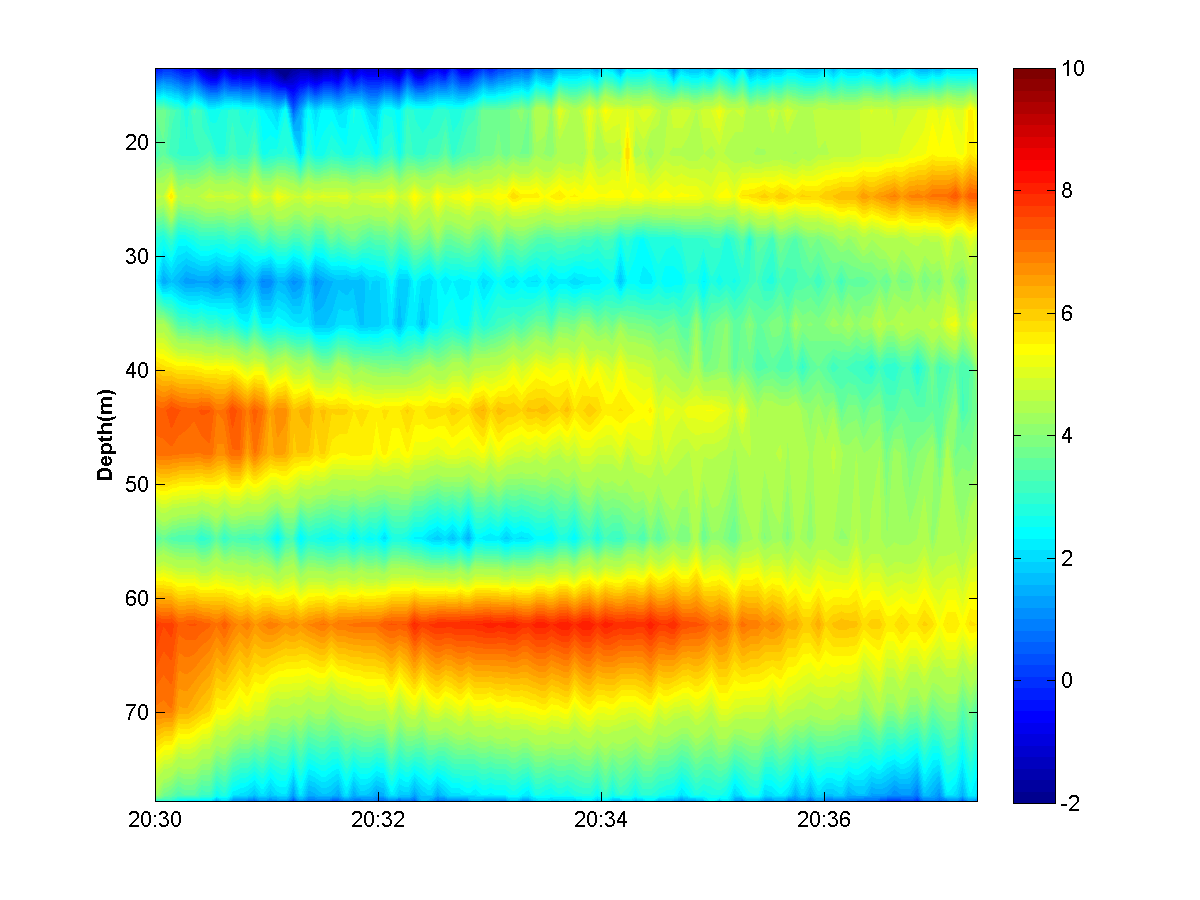
\includegraphics[width=0.3\textwidth,height=0.1\textwidth]{0817_2030_vla.png}
 % 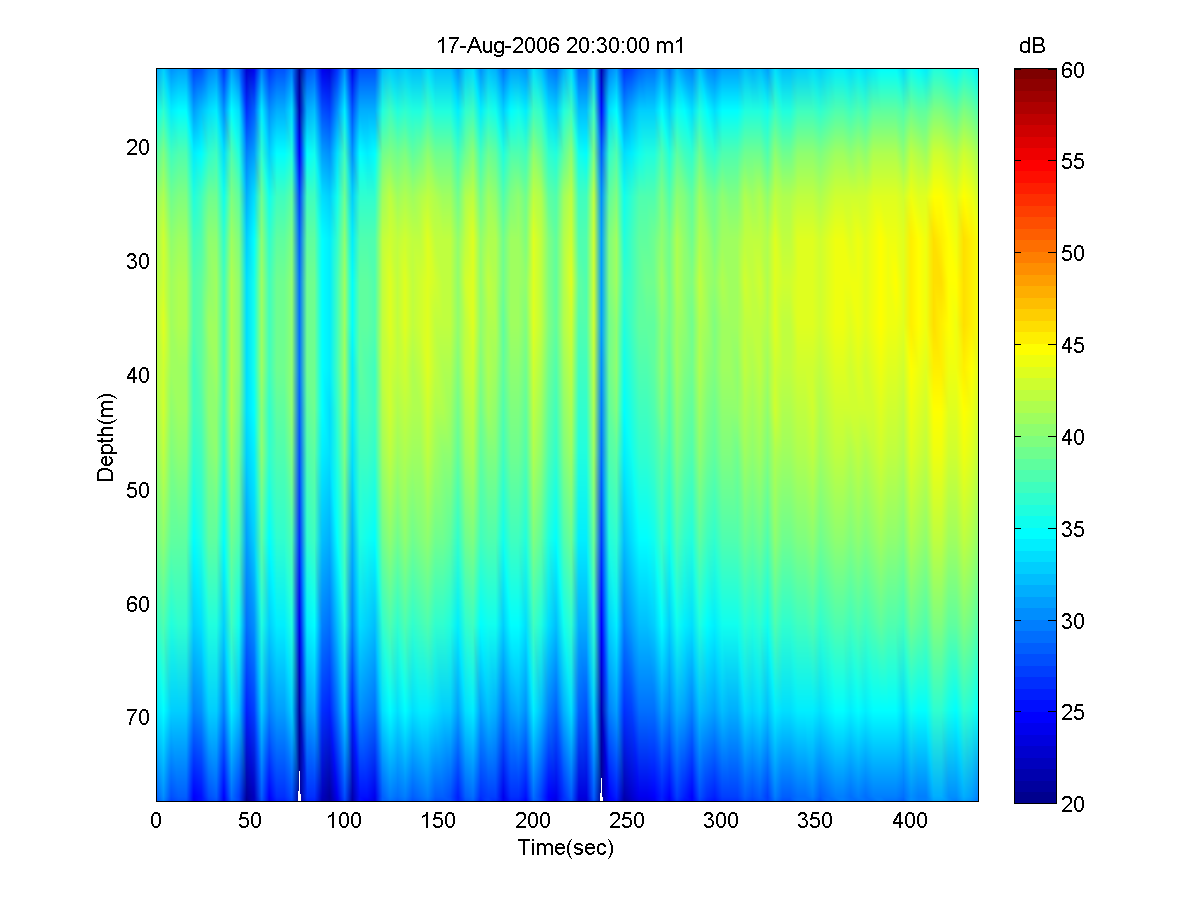
\includegraphics[width=0.3\textwidth,height=0.1\textwidth]{nrl_200608172030_m1.png}
 % 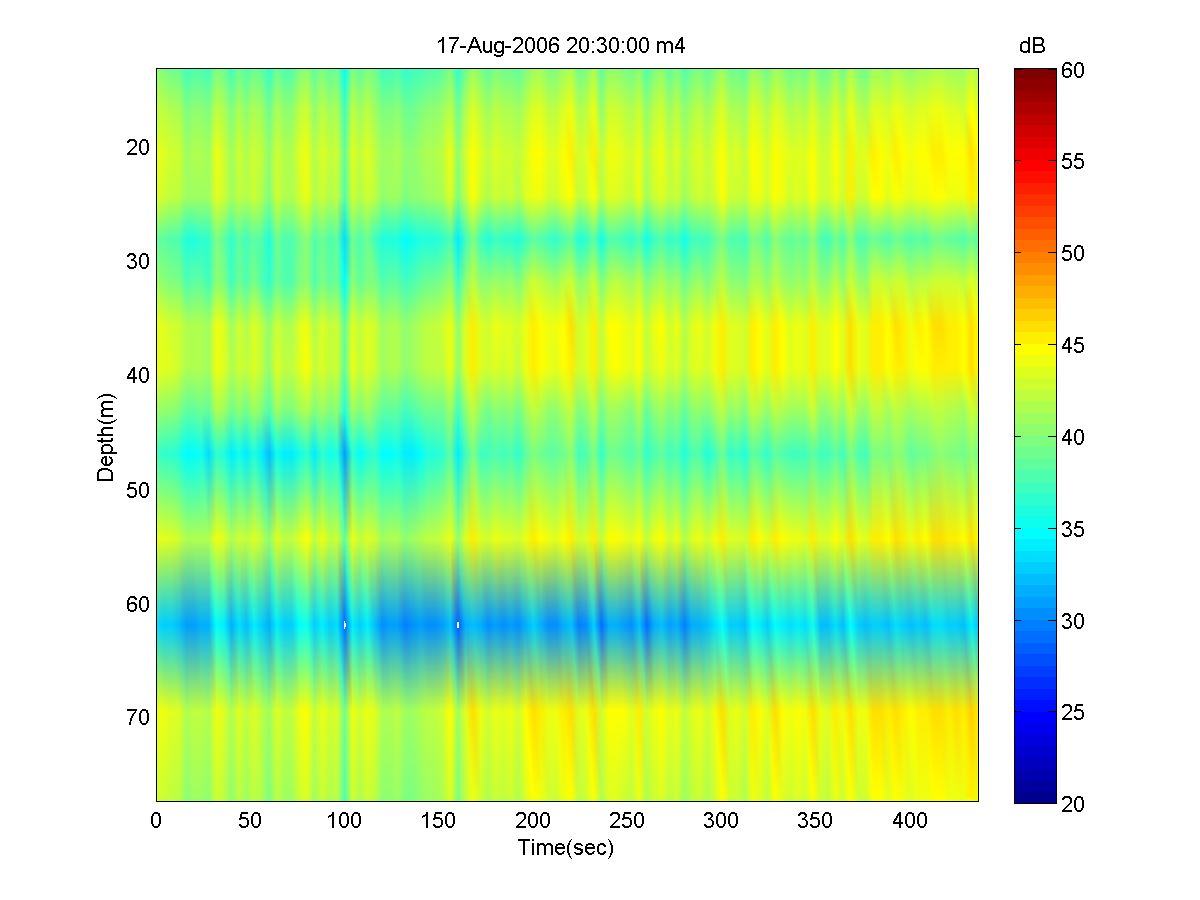
\includegraphics[width=0.3\textwidth,height=0.1\textwidth]{nrl_200608172030_m4.png}\\
 % 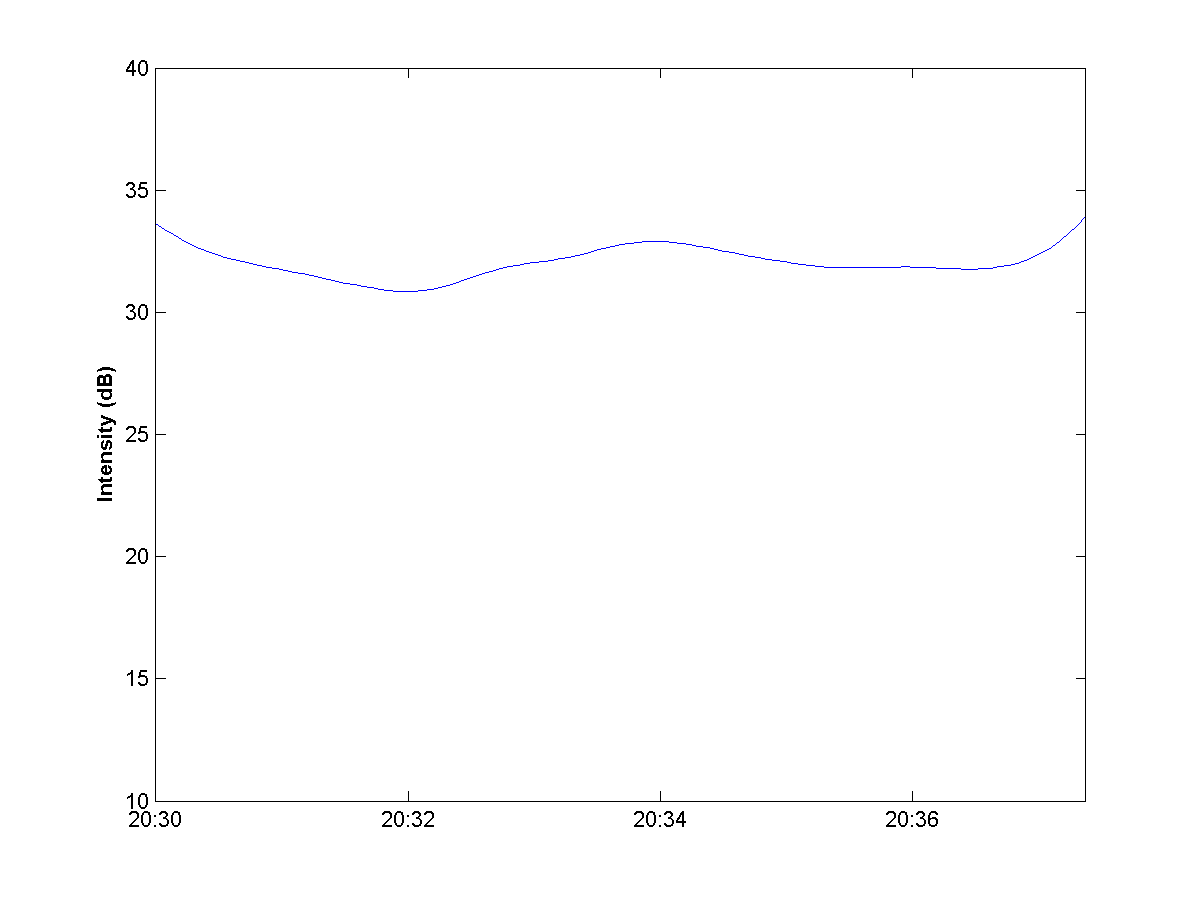
\includegraphics[width=0.3\textwidth,height=0.1\textwidth]{0817_2030_eng.png}
 % 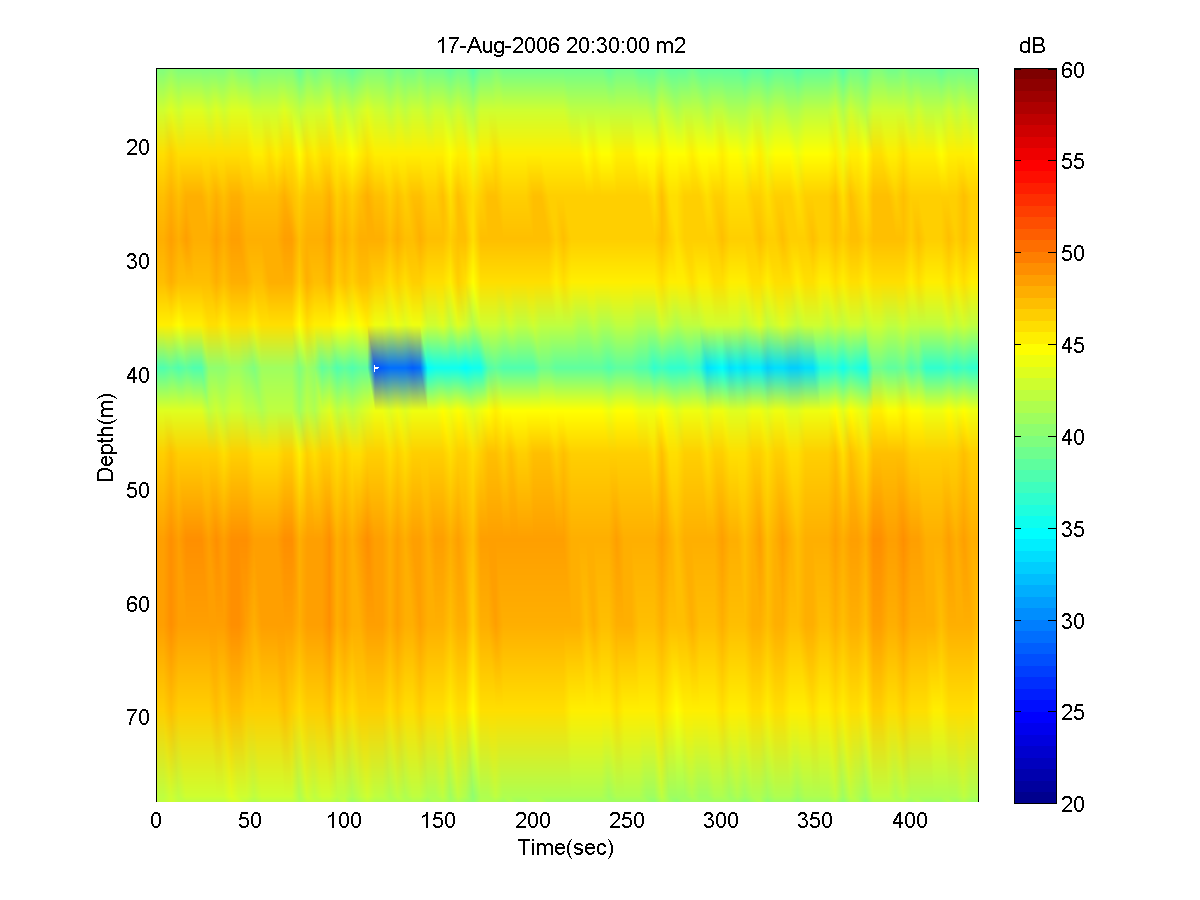
\includegraphics[width=0.3\textwidth,height=0.1\textwidth]{nrl_200608172030_m2.png}
  %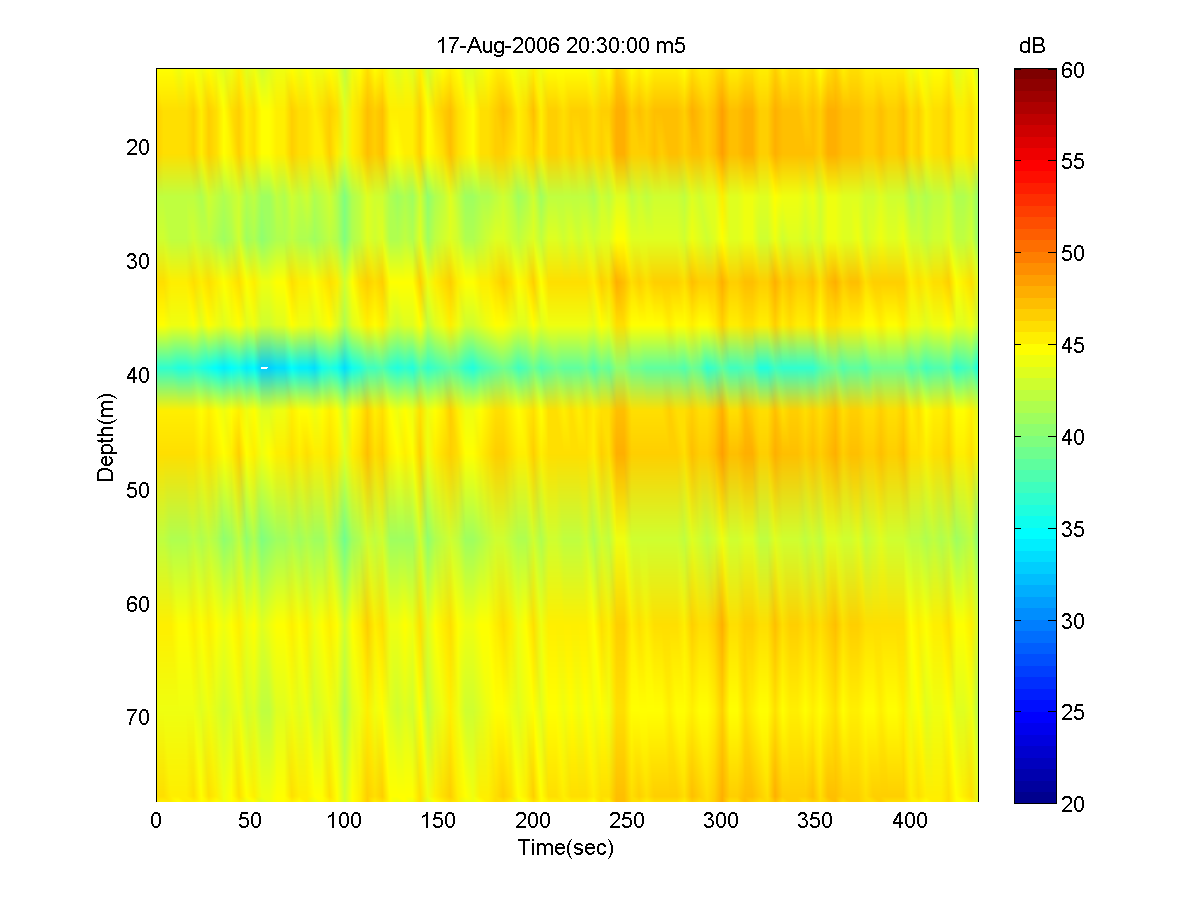
\includegraphics[width=0.3\textwidth,height=0.1\textwidth]{nrl_200608172030_m5.png}\\
  %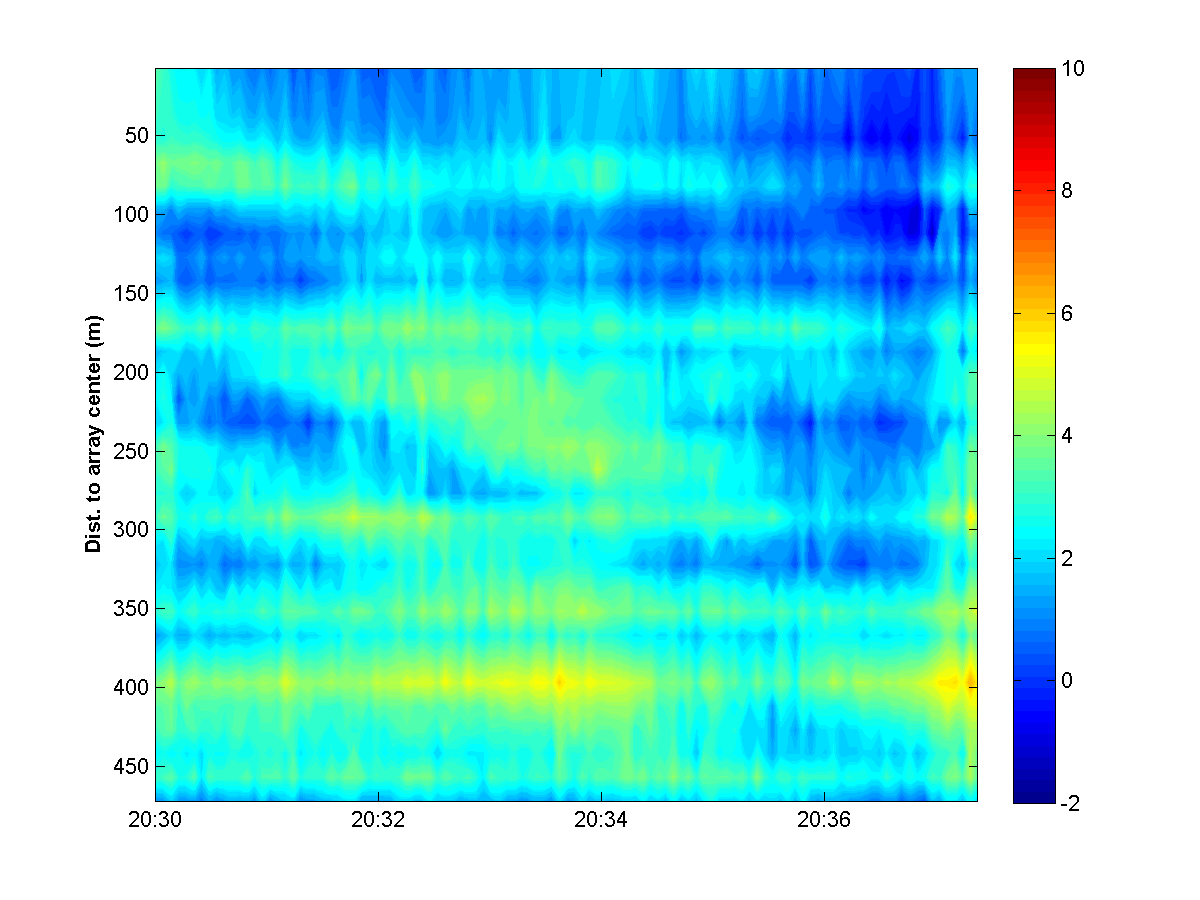
\includegraphics[width=0.3\textwidth,height=0.1\textwidth]{0817_2030_hla.png}
  %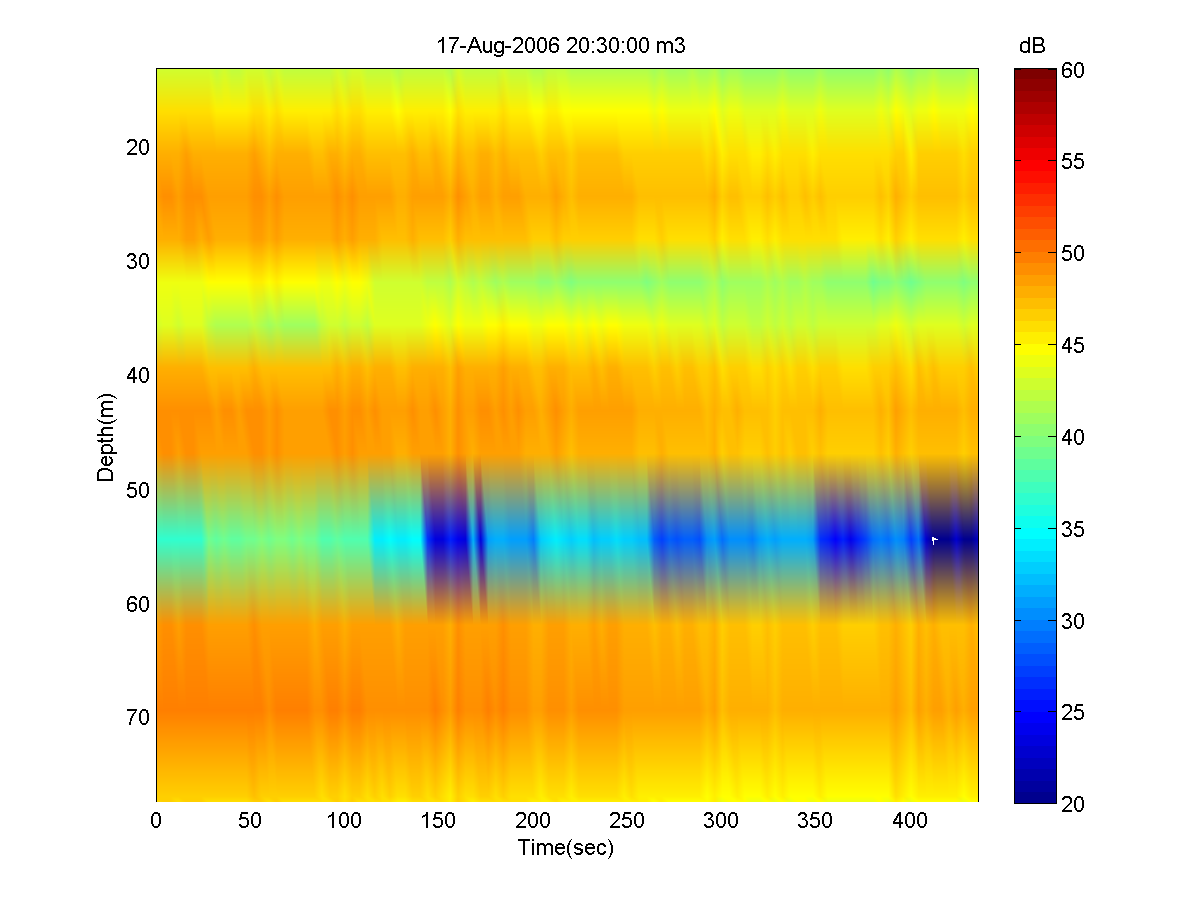
\includegraphics[width=0.3\textwidth,height=0.1\textwidth]{nrl_200608172030_m3.png}
  %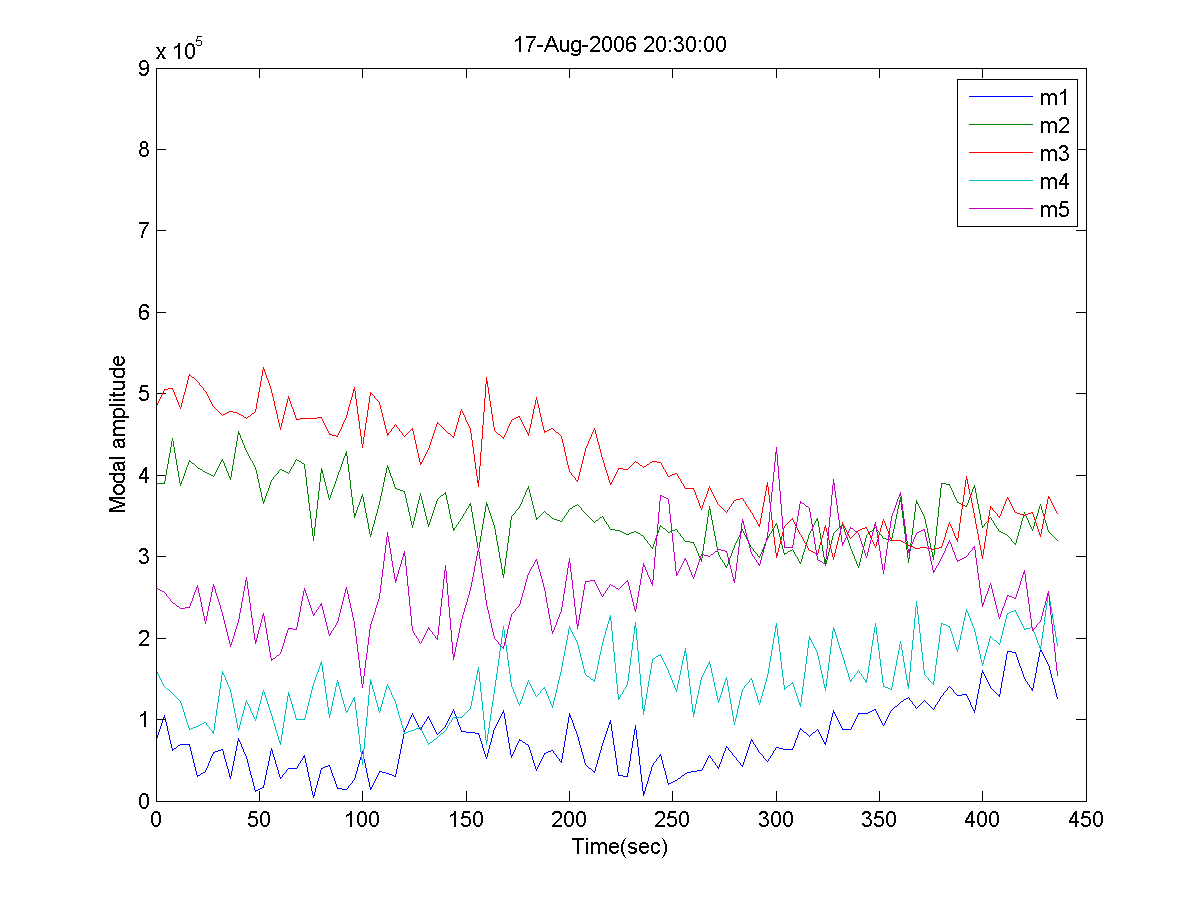
\includegraphics[width=0.3\textwidth,height=0.1\textwidth]{nrl_ma_200608172030.png}\\
 % \end{tabular}
  %\caption{Received signal on Shark array from Aug.17 20:30GMT to 20:37GMT. Left column, from top to bottom: signal on VLA, VLA signal intensity, signal on HLA; middle column: mode 1-3; right column: mode 4, 5, and modal amplitudes.}\label{fig:m2030}
%\end{figure}

%
%\subsection{21:00GMT-21:07GMT}
%
%Figure\ref{fig:r2100} shows the radar image at 21:00GMT. The ISWs is still about
%1km away from the VLA, and very similar to the previous time period
%(20:30GMT - 20:37GMT), only very little fluctuation of the total
%intensity is shown (Fig.\ref{fig:a2100}). On the modal decomposition plot (Fig.\ref{fig:m2100}), the 3rd mode
%grows while the other modes decrease to various extends. The modal
%coupling might cause this as well.

%\begin{figure}[H]
 % \centering
  %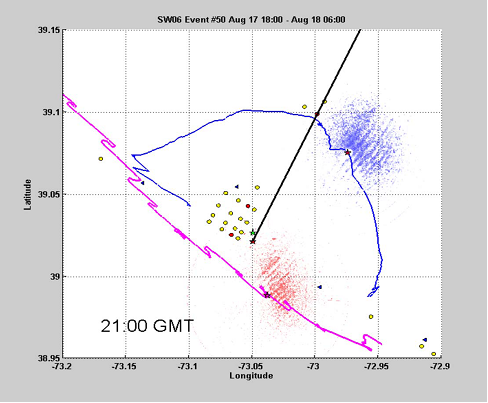
\includegraphics[width=0.5\textwidth]{radar2100.png}
 % \caption{Radar image of ISW at 21:00GMT}\label{fig:r2100}
%\end{figure}
%
%\begin{figure}[H]
%  \centering
%  \begin{tabular}{l}
%  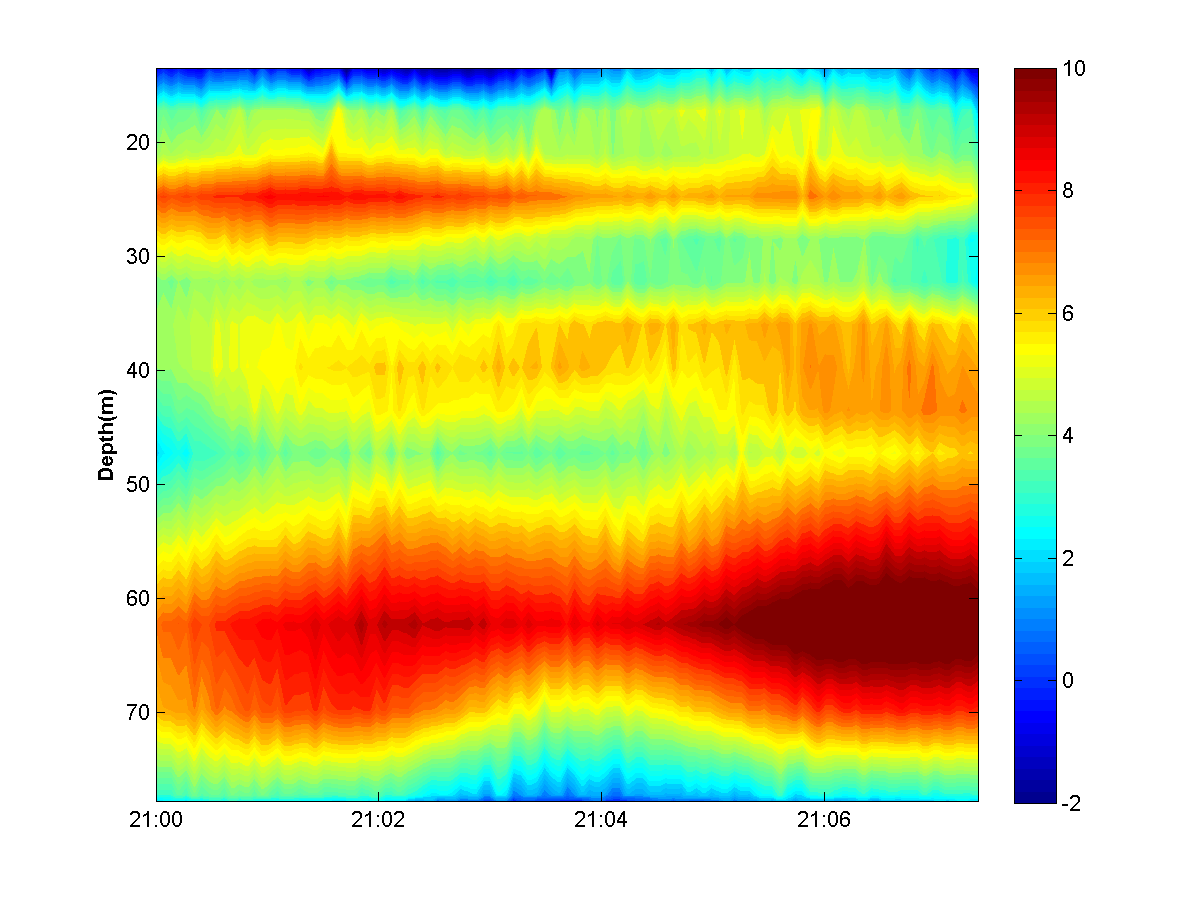
\includegraphics[width=0.5\textwidth,height=0.2\textwidth]{0817_2100_vla.png}\\
%  \ 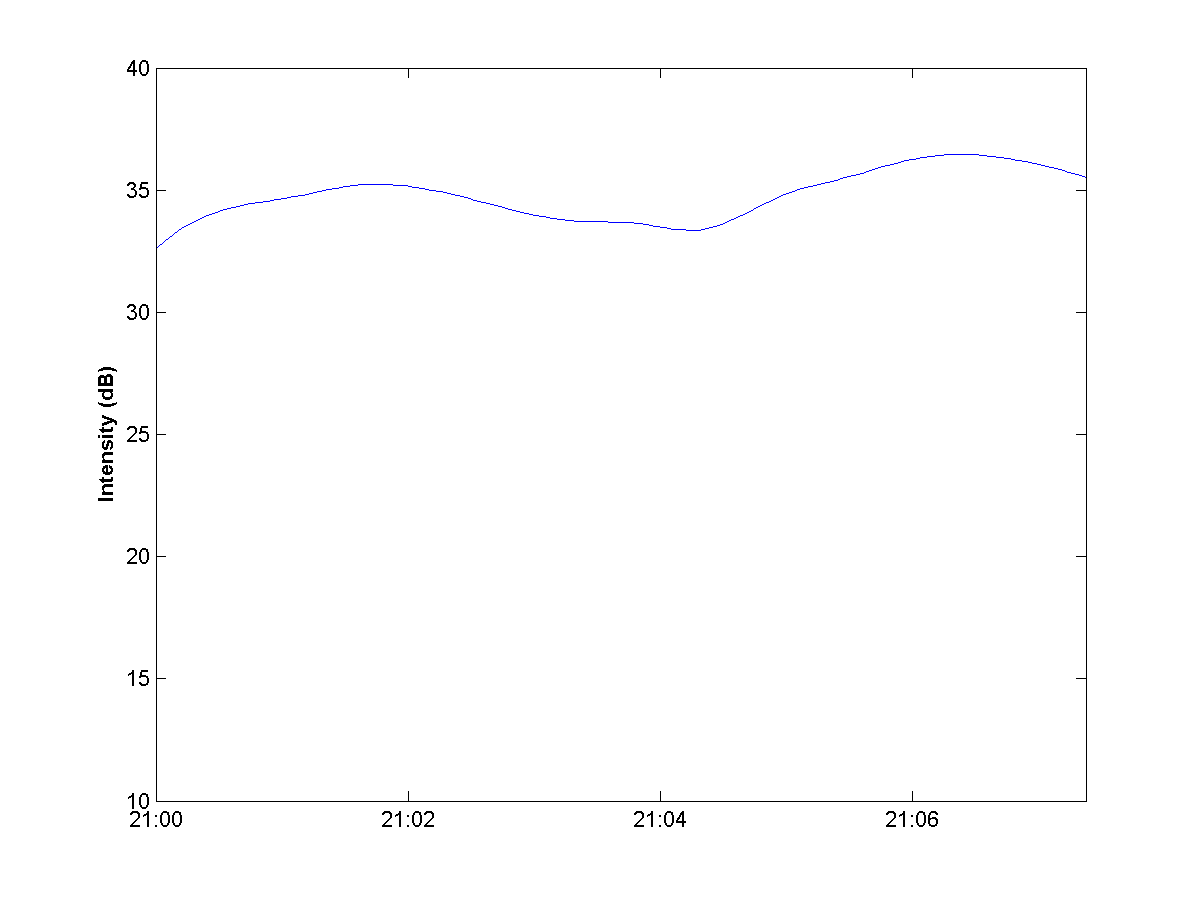
\includegraphics[width=0.44\textwidth,height=0.2\textwidth]{0817_2100_eng.png}\\
%  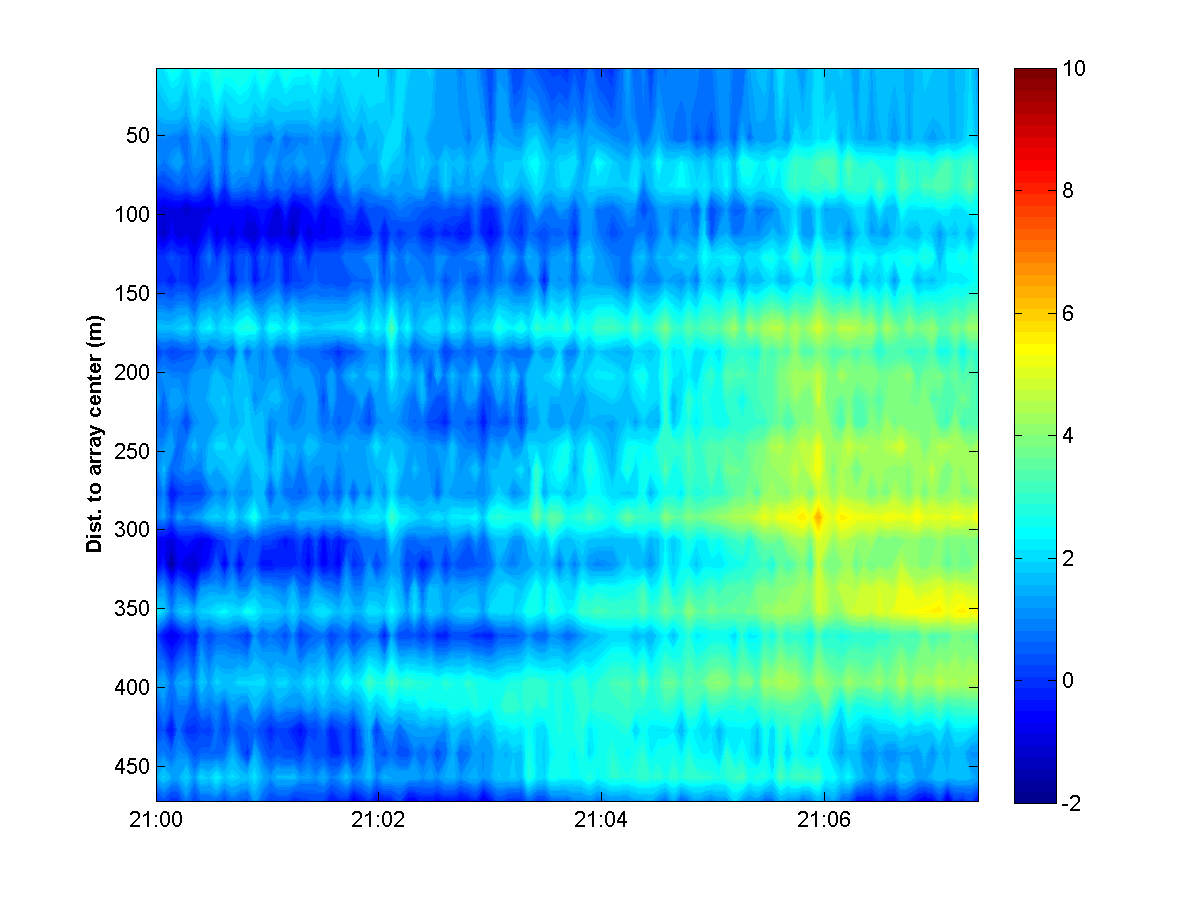
\includegraphics[width=0.5\textwidth,height=0.2\textwidth]{0817_2100_hla.png}\\
%  \end{tabular}
%  \caption{Received signal on Shark VLA (top), HLA (bottom) and signal intensity (middle) from Aug.17 21:00GMT to 21:07GMT }\label{fig:a2100}
%\end{figure}
%
%\begin{figure}[H]
%  \centering
%  \begin{tabular}{cc}
%  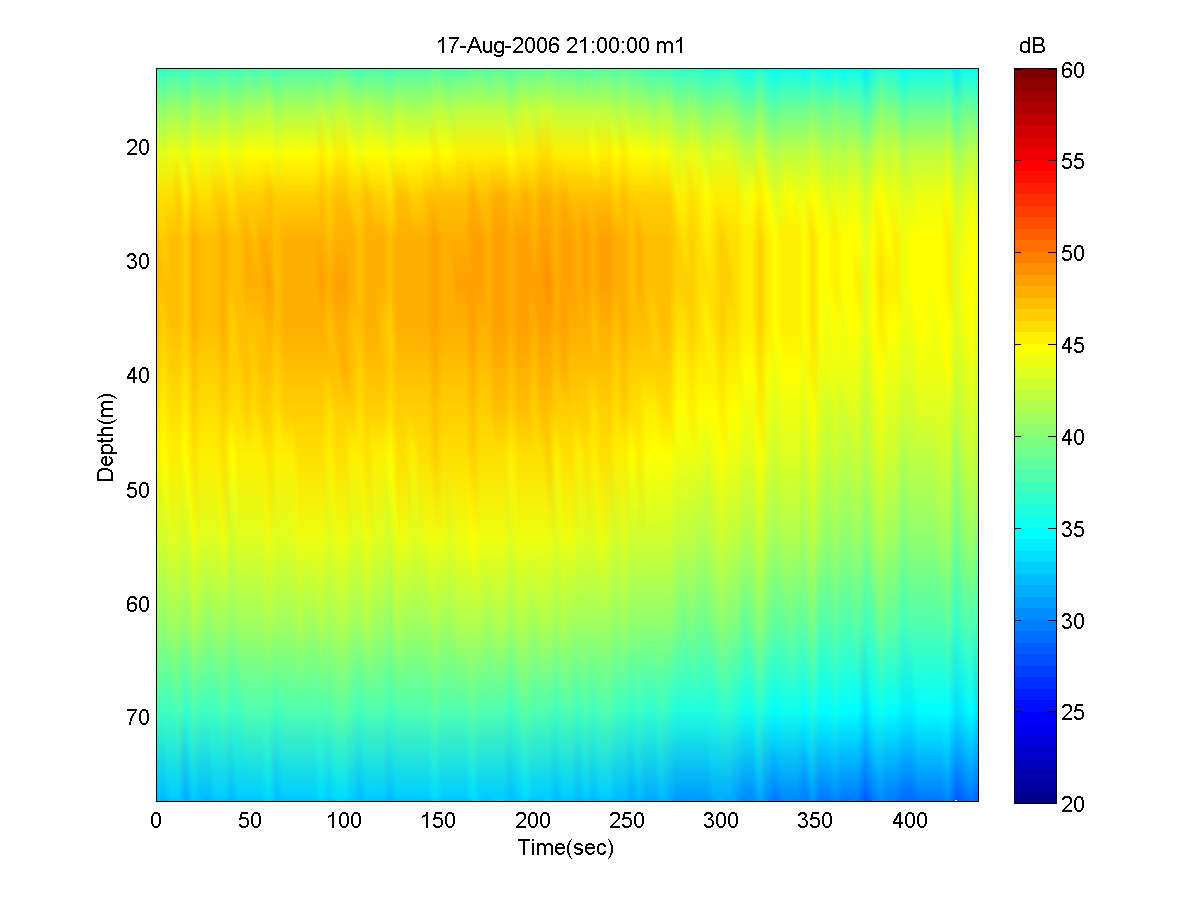
\includegraphics[width=0.5\textwidth,height=0.2\textwidth]{nrl_200608172100_m1.png}
%  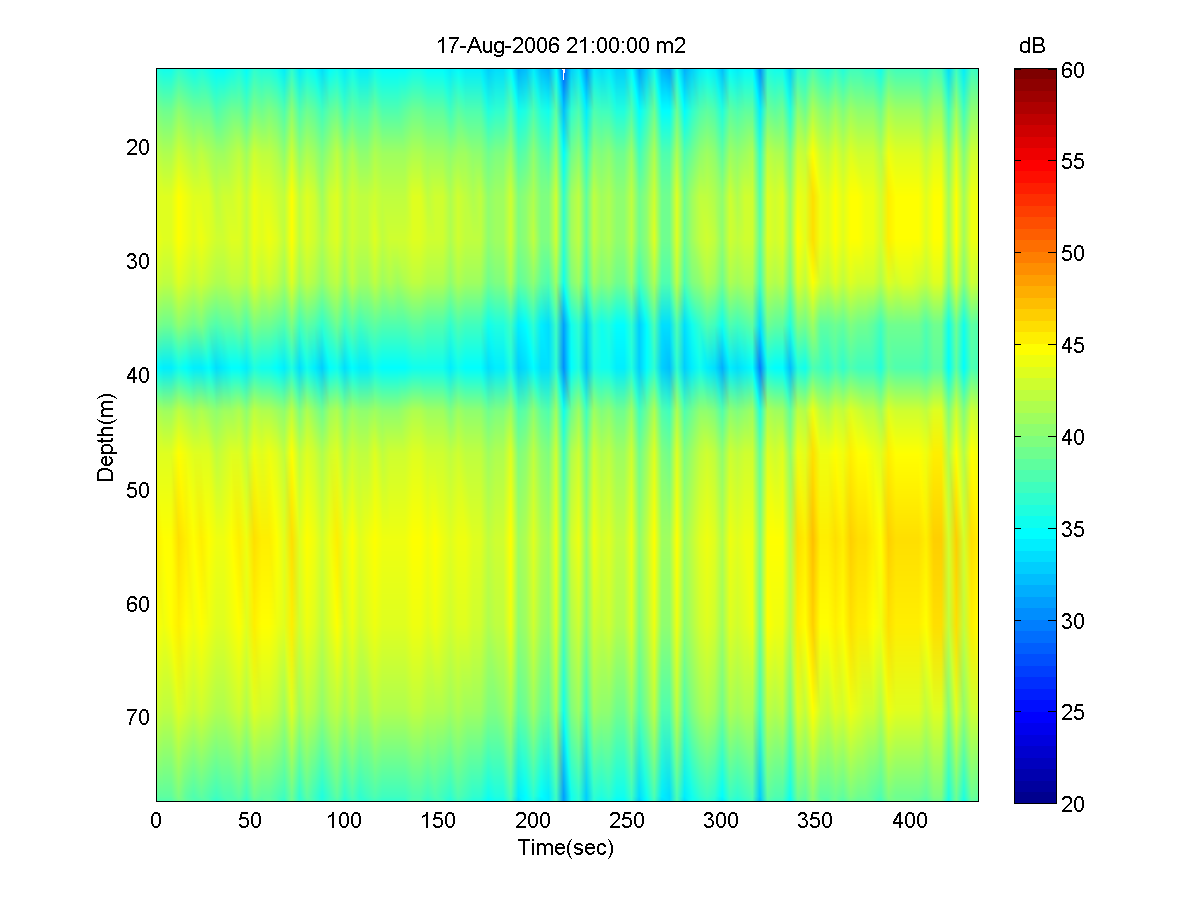
\includegraphics[width=0.5\textwidth,height=0.2\textwidth]{nrl_200608172100_m2.png}\\
%  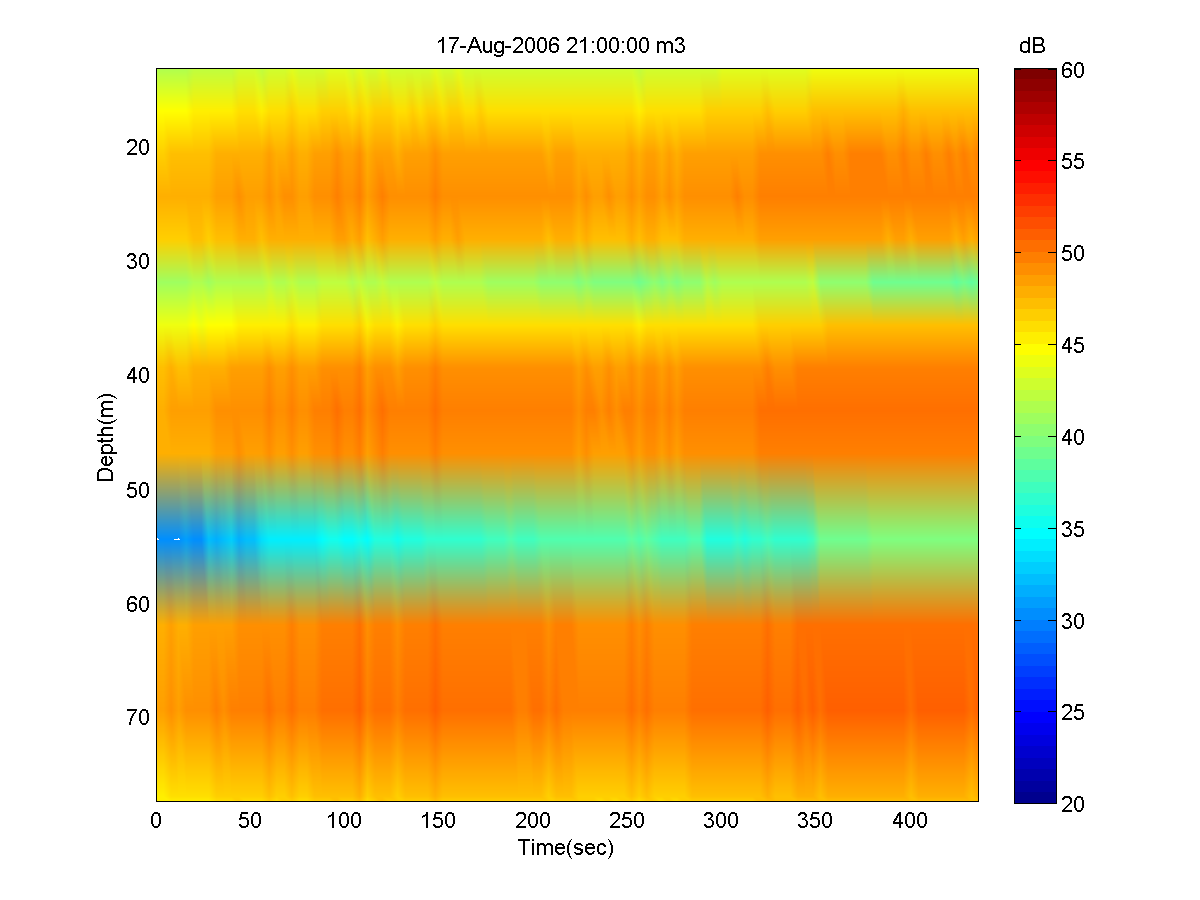
\includegraphics[width=0.5\textwidth,height=0.2\textwidth]{nrl_200608172100_m3.png}
%  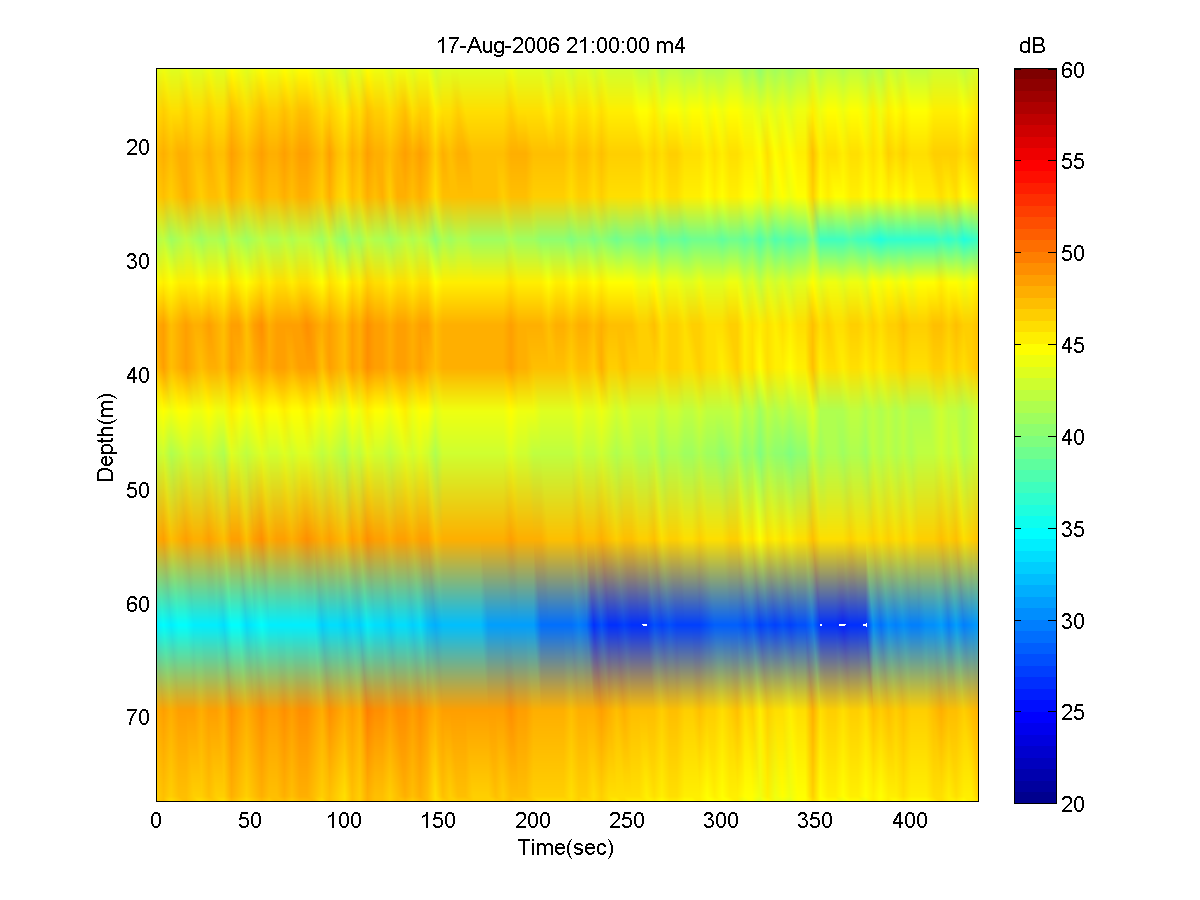
\includegraphics[width=0.5\textwidth,height=0.2\textwidth]{nrl_200608172100_m4.png}\\
%  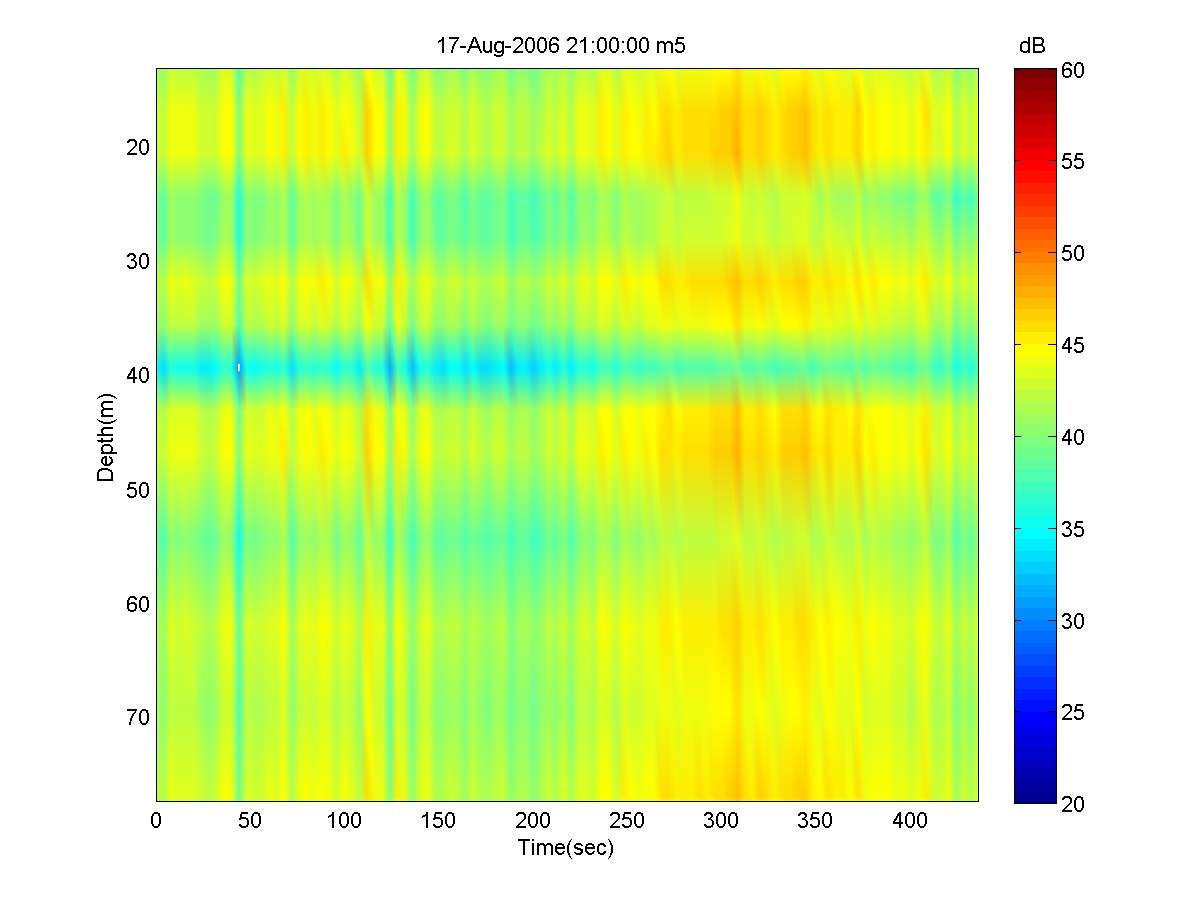
\includegraphics[width=0.5\textwidth,height=0.2\textwidth]{nrl_200608172100_m5.png}
%  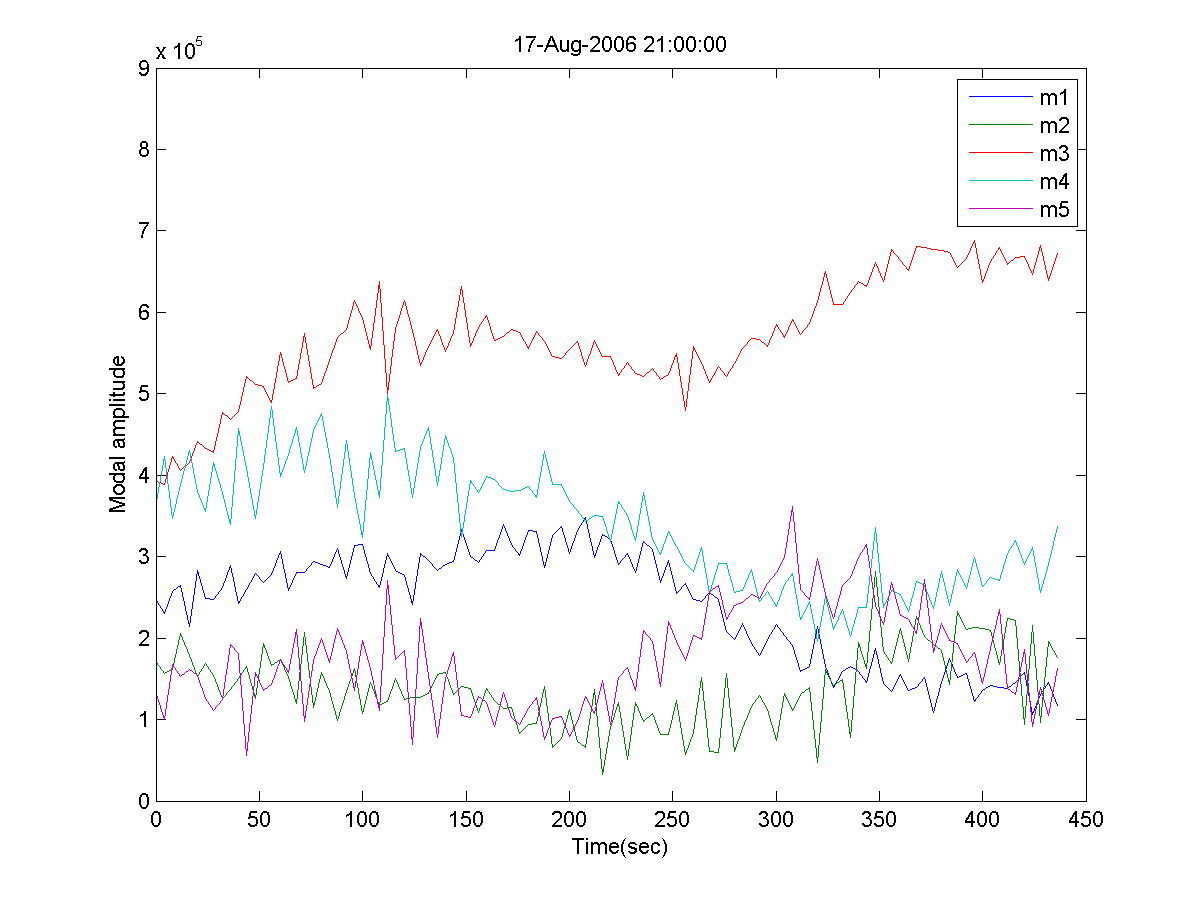
\includegraphics[width=0.5\textwidth,height=0.2\textwidth]{nrl_ma_200608172100.png}\\
%  \end{tabular}
%  \caption{Modal decomposition and amplitude of the signal received on Shark VLA from Aug.17 21:00GMT to 21:07GMT }\label{fig:m2100}
%\end{figure}


%\begin{figure}
 % \centering
  %\begin{tabular}{lrr}
  %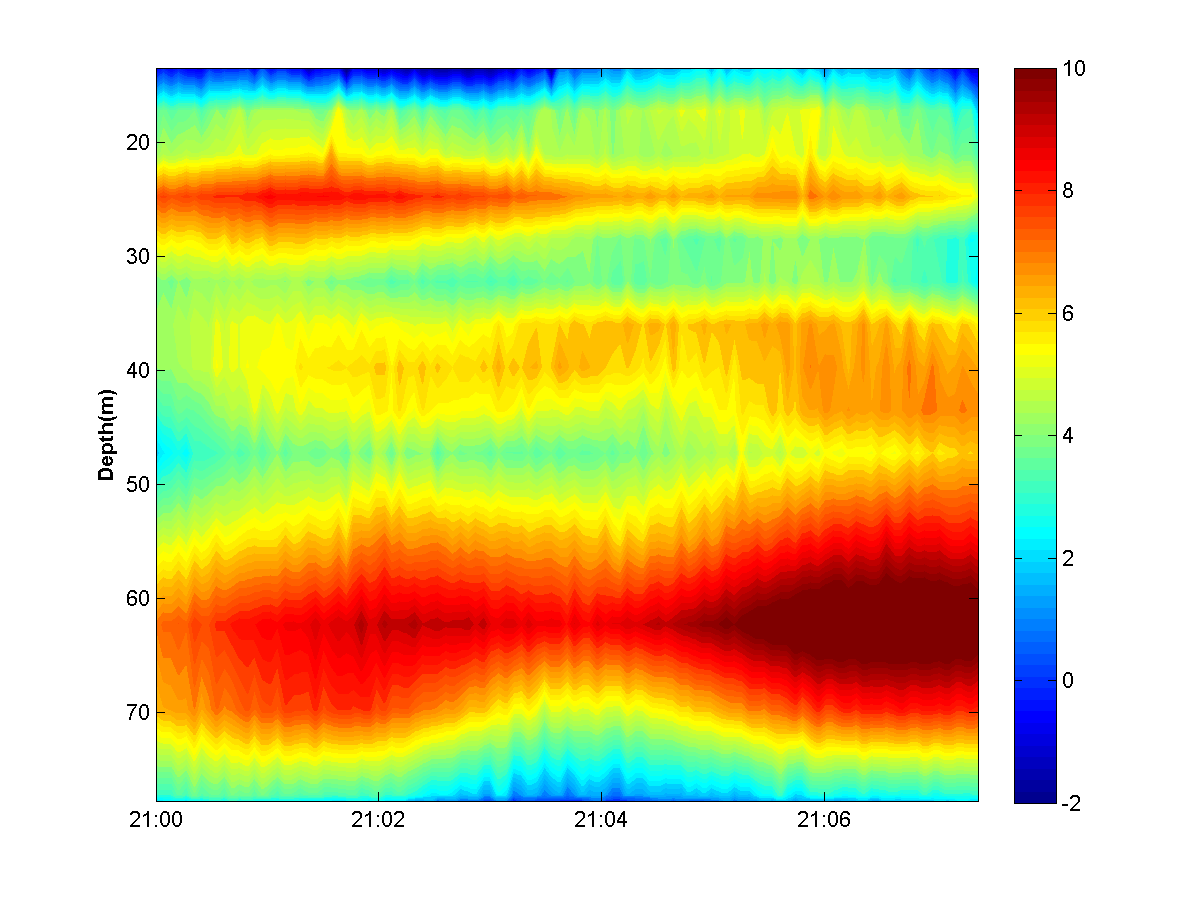
\includegraphics[width=0.3\textwidth,height=0.1\textwidth]{0817_2100_vla.png}
  %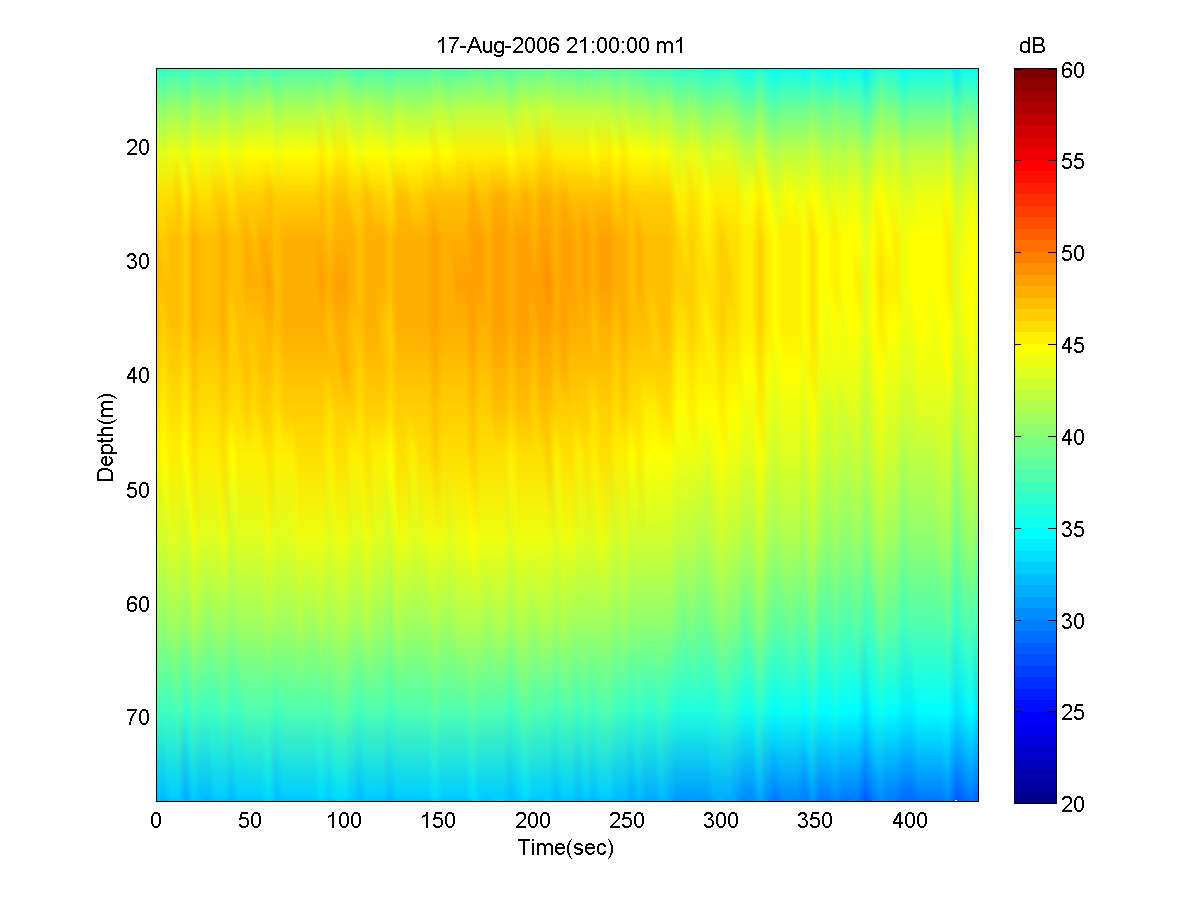
\includegraphics[width=0.3\textwidth,height=0.1\textwidth]{nrl_200608172100_m1.png}
  %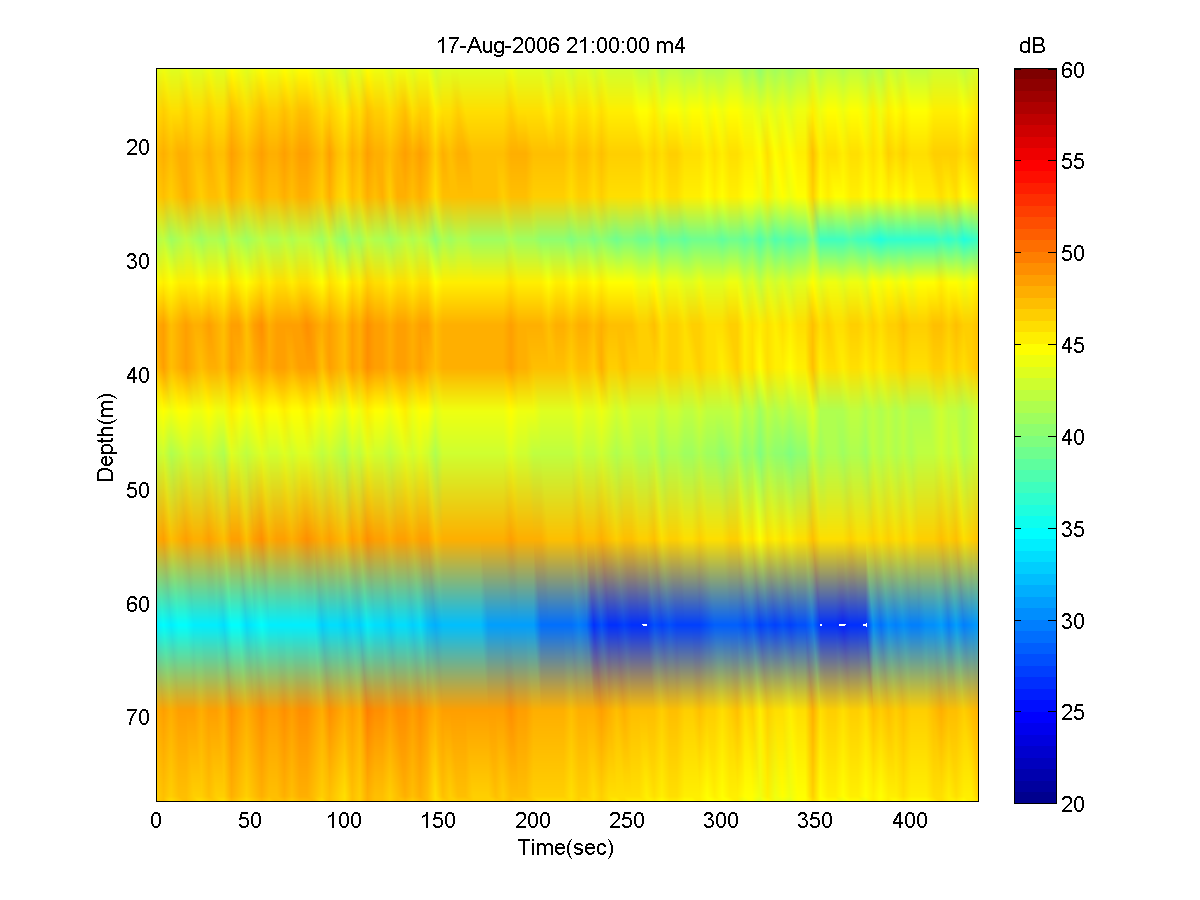
\includegraphics[width=0.3\textwidth,height=0.1\textwidth]{nrl_200608172100_m4.png}\\
  %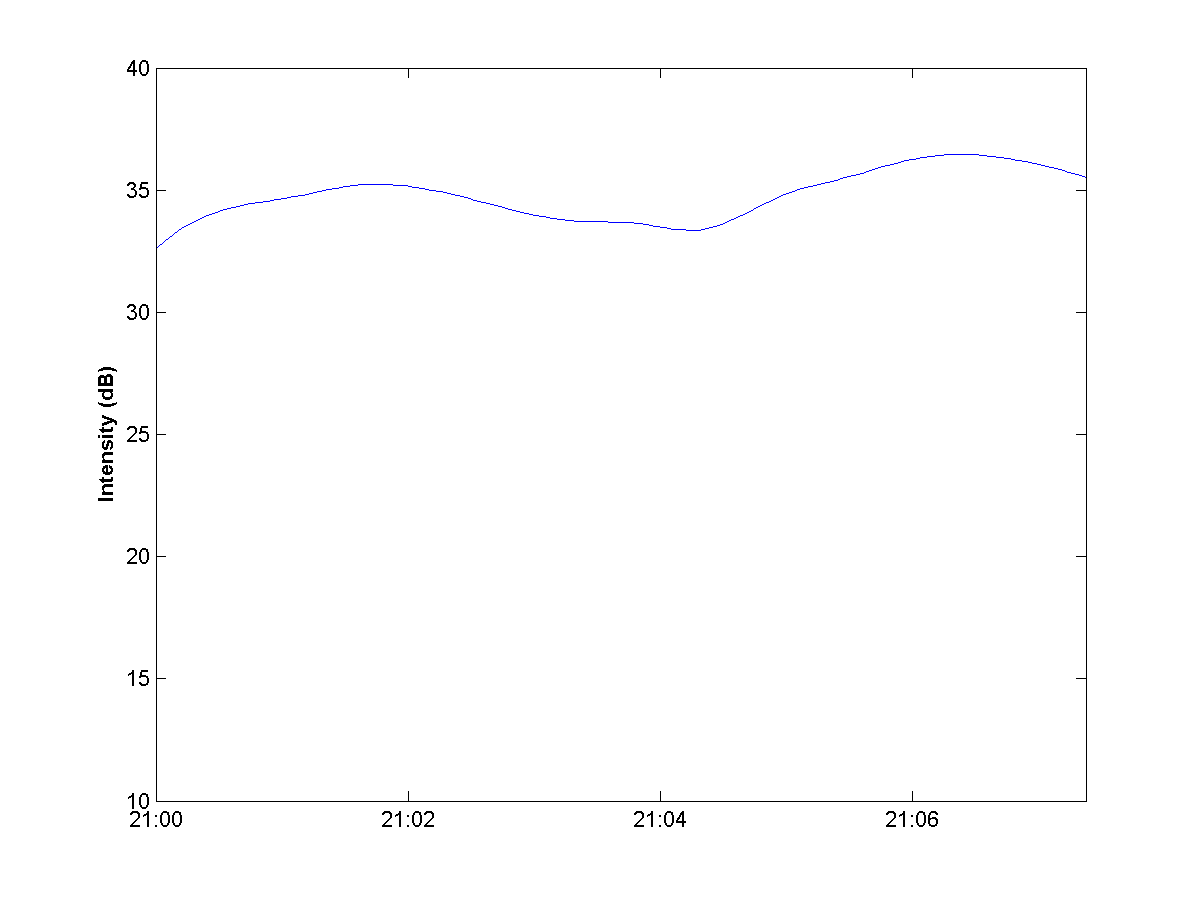
\includegraphics[width=0.3\textwidth,height=0.1\textwidth]{0817_2100_eng.png}
  %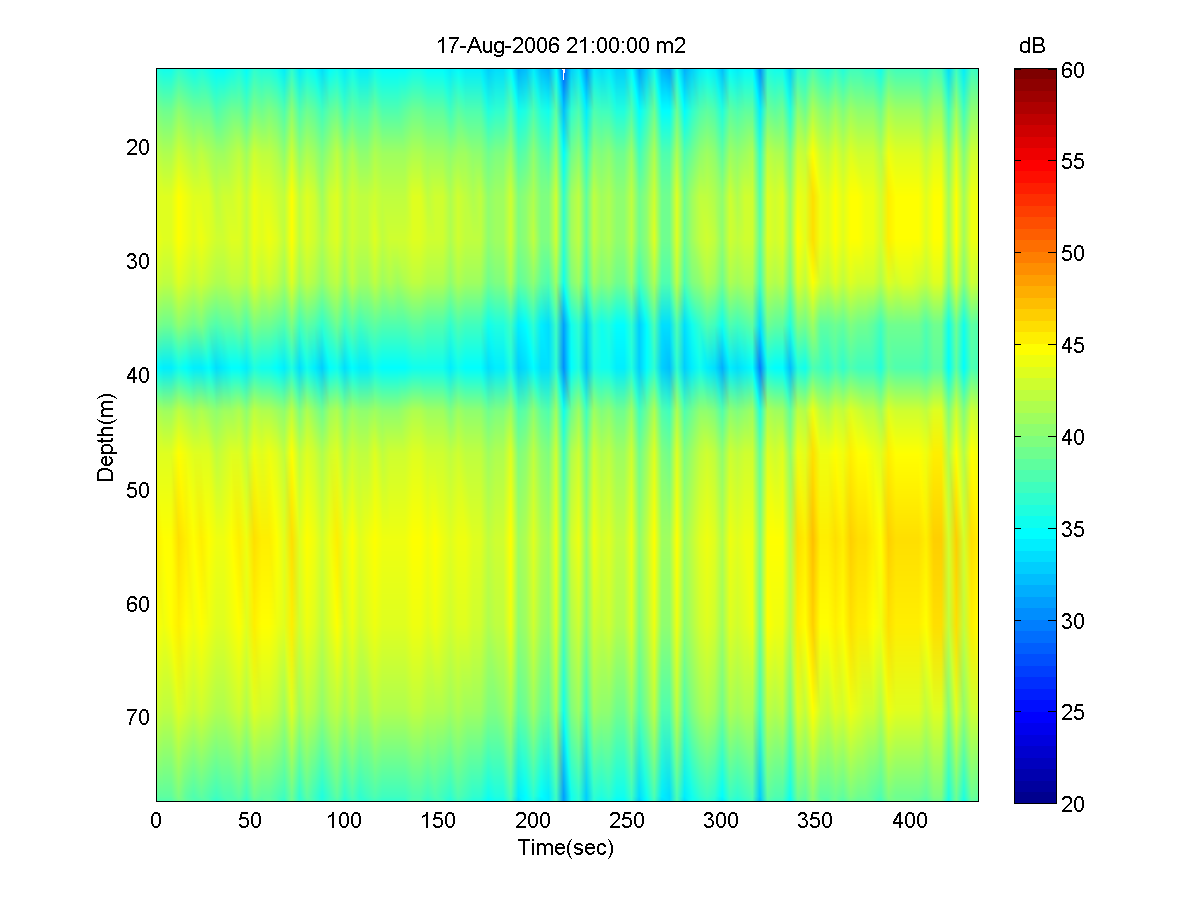
\includegraphics[width=0.3\textwidth,height=0.1\textwidth]{nrl_200608172100_m2.png}
  %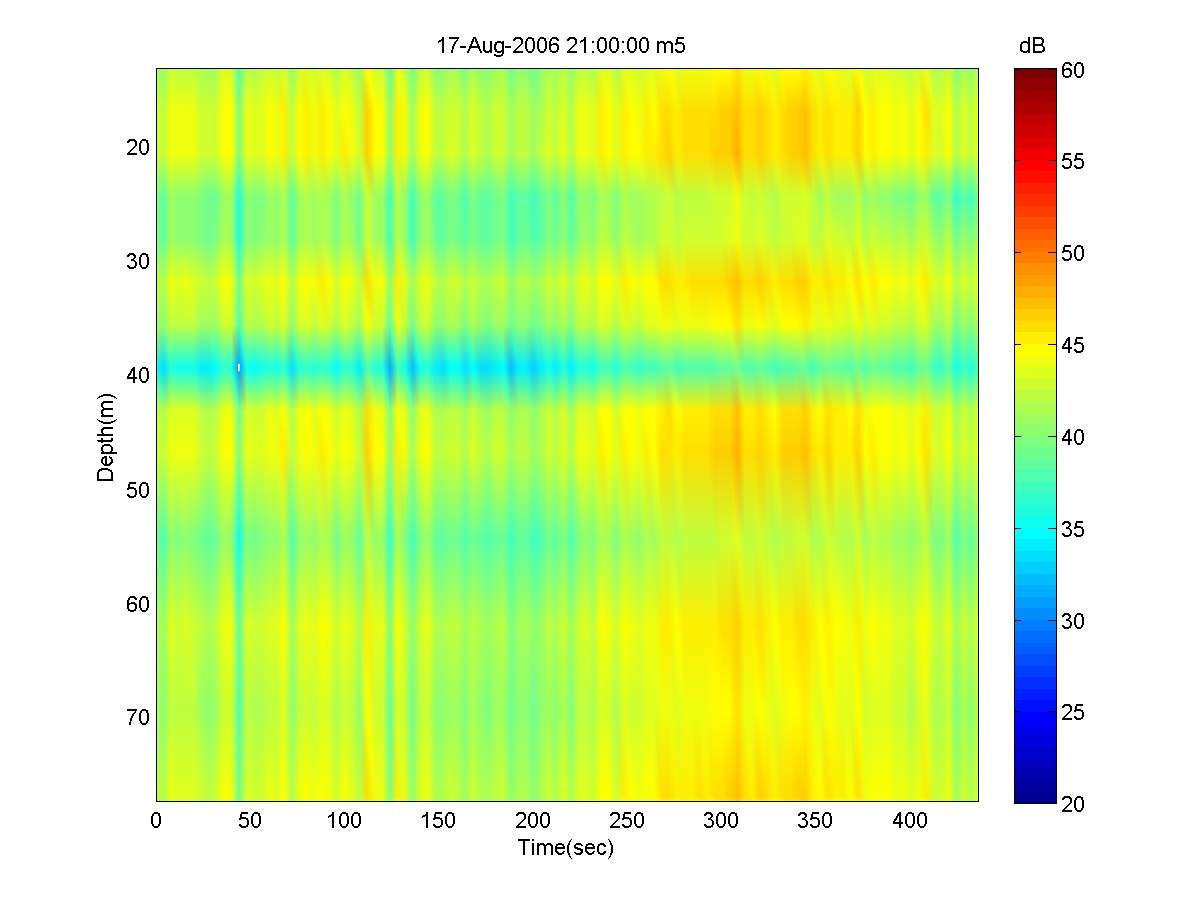
\includegraphics[width=0.3\textwidth,height=0.1\textwidth]{nrl_200608172100_m5.png}\\
  %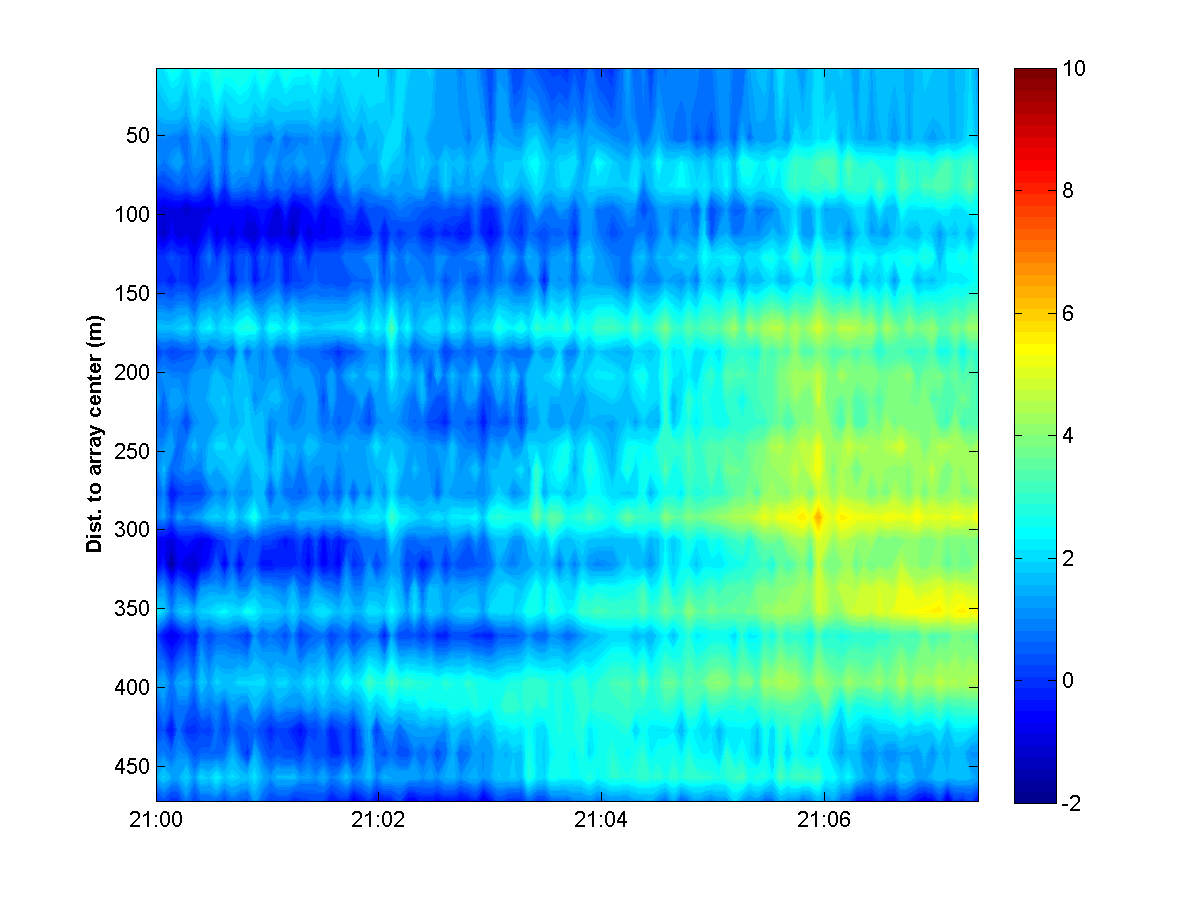
\includegraphics[width=0.3\textwidth,height=0.1\textwidth]{0817_2100_hla.png}
  %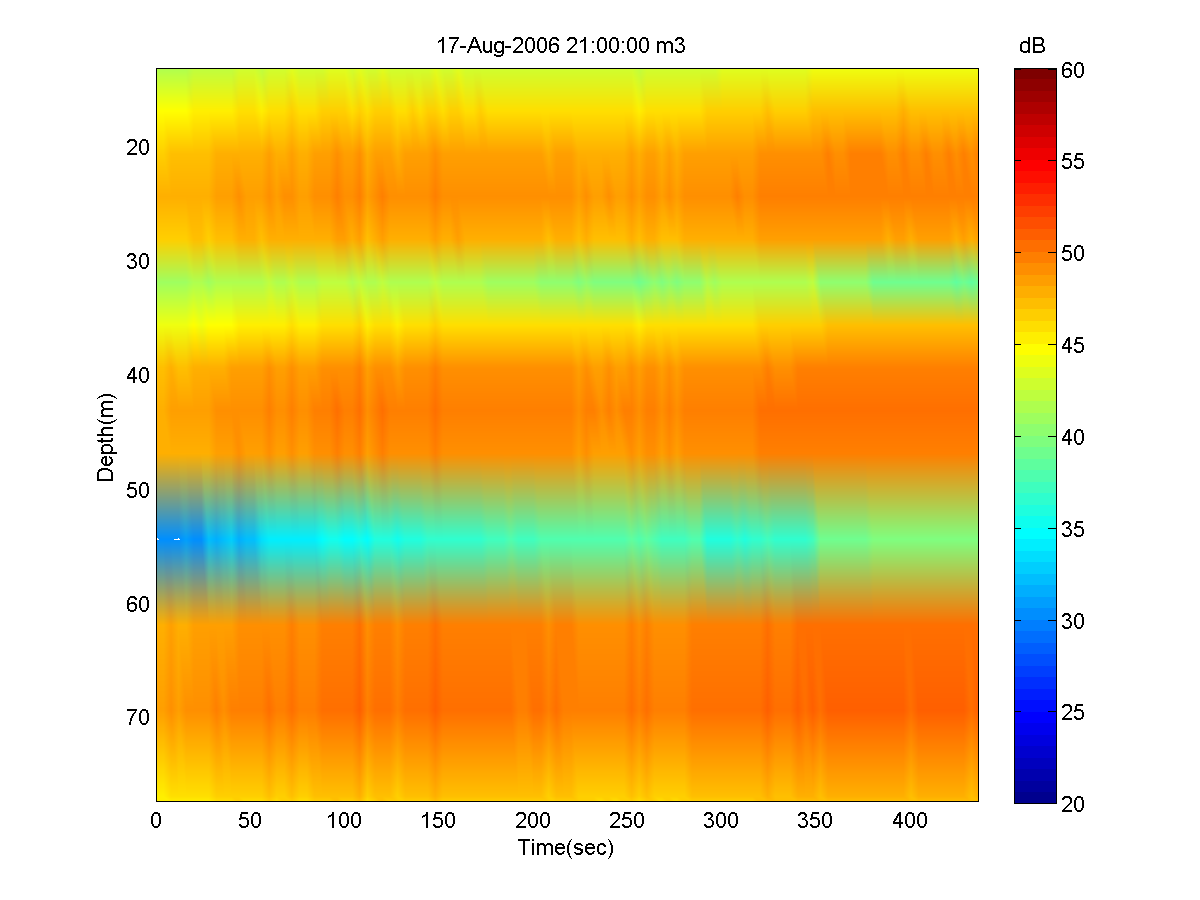
\includegraphics[width=0.3\textwidth,height=0.1\textwidth]{nrl_200608172100_m3.png}
  %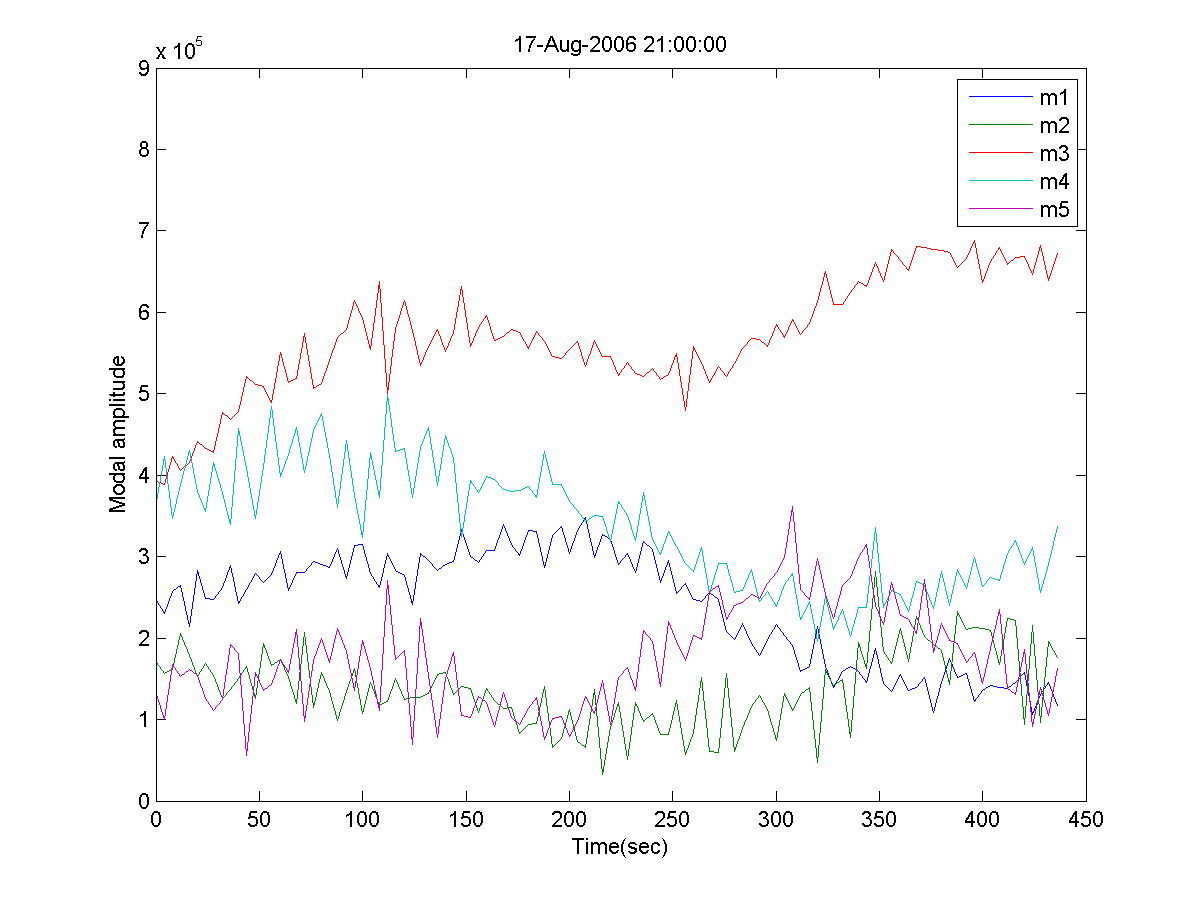
\includegraphics[width=0.3\textwidth,height=0.1\textwidth]{nrl_ma_200608172100.png}\\
  %\end{tabular}
  %\caption{Received signal on Shark array from Aug.17 21:00GMT to 21:07GMT. Left column, from top to bottom: signal on VLA, VLA signal intensity, signal on HLA; middle column: mode 1-3; right column: mode 4, 5, and modal amplitudes.}\label{fig:m2100}
%\end{figure}
\subsection{Phase II: 21:30-21:37GMT}
Phase II is of particular interests here because from the internal wave map (Fig. \ref{fig:r2130_i}), the leading front of the IW packet is still at about 1km away from the Shark VLA at the end of the transmission session (21:37GMT), but its impact on the acoustic propagation can be seen on the received signal on the Shark array. The impact, which is similar to the optical Lloyd mirror effect, will be further analyzed in chapter \ref{ch:analysis}.
Figure \ref{fig:r2130_i} shows the radar image and the interpolated temperature field at 21:30GMT. The received signal on Shark VLA and HLA shows a clear contrast between the first and second halves of this transmission. During the first half, the signal continues the steady characteristic from phase I. When the IW moves closer in the second half, the acoustic signal changes to a oscillating two-strip pattern. 
%
%Radar image shows the major ISW reaches the VLA at about 21:37GMT,
%but the signal received on SHARK VLA and HLA shows the effects of
%ISW on the acoustic propagation starts a bit earlier at about
%21:33GMT when the HLA shows the slope caused by the movement of the
%ISW. A 5dB dip on the total intensity plot implies the energy could
%be transferred out of the VLA plane. Mode 1 and 2 are steady and
%strong when pushed to the deeper water by the downward movement of
%the thermocline. On the other hand, mode 3, 4 and 5 show strong
%(~8dB) and fast(period = 50sec) oscillation starting about 21:33GMT,
%confirming the effects of ISW on acoustic propagation.



%\begin{figure}[H]
%  \centering
%  \begin{tabular}{l}
%  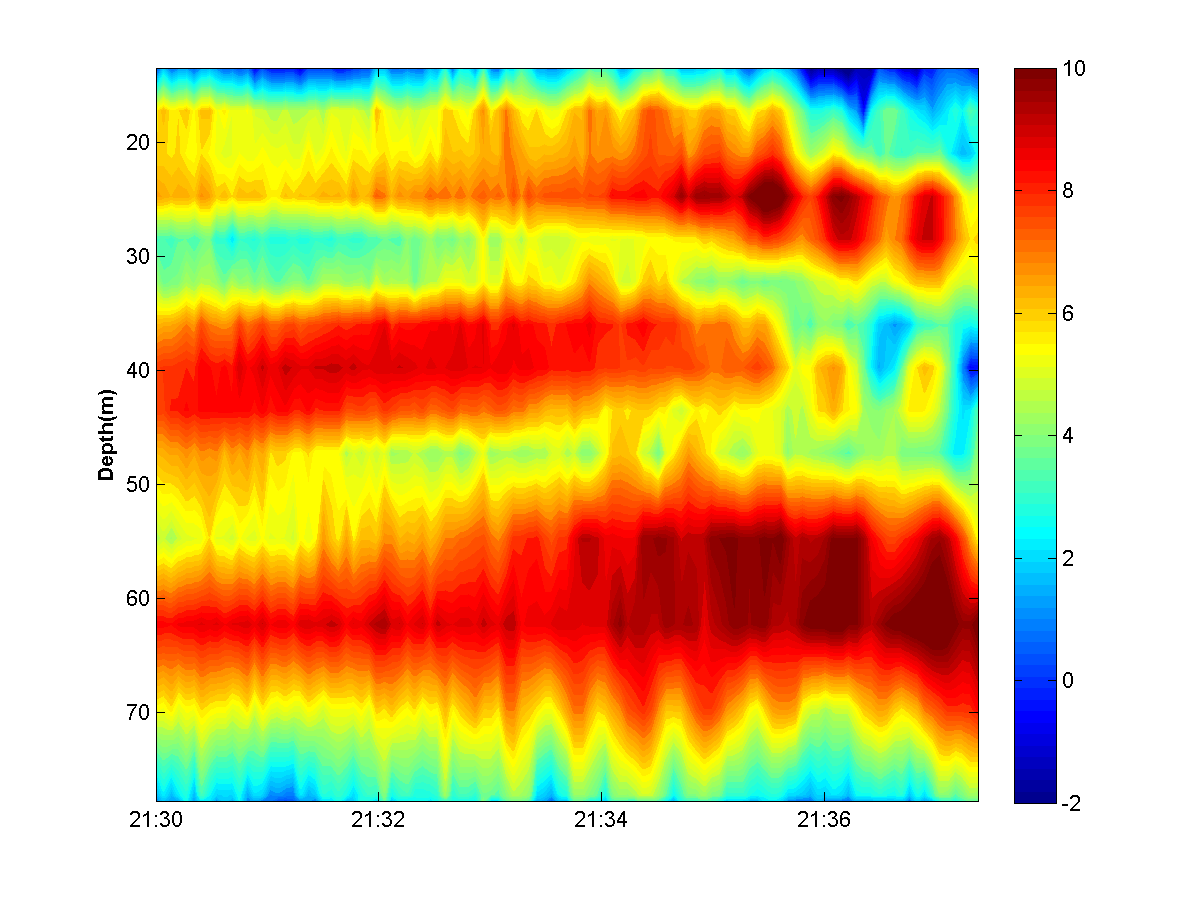
\includegraphics[width=0.5\textwidth,height=0.2\textwidth]{0817_2130_vla.png}\\
%  \ 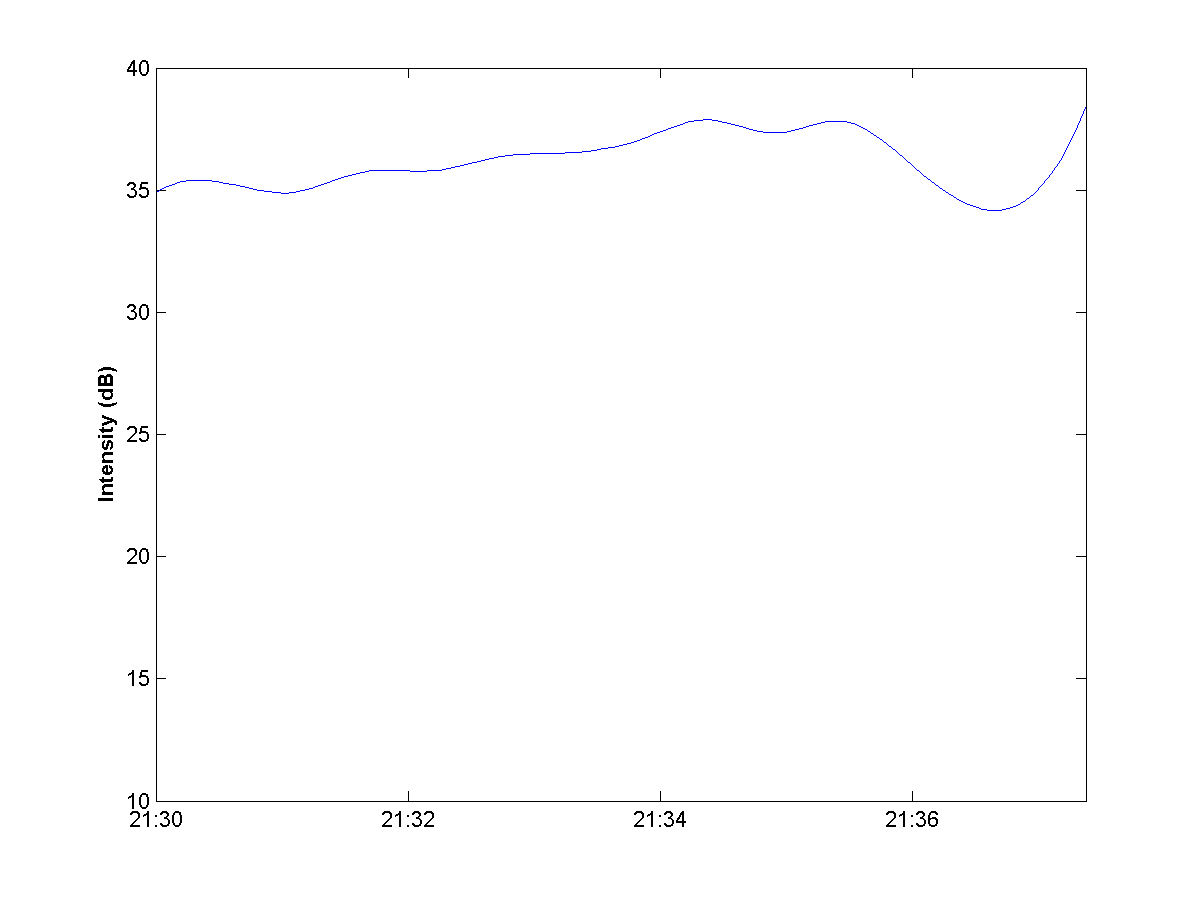
\includegraphics[width=0.44\textwidth,height=0.2\textwidth]{0817_2130_eng.png}\\
%  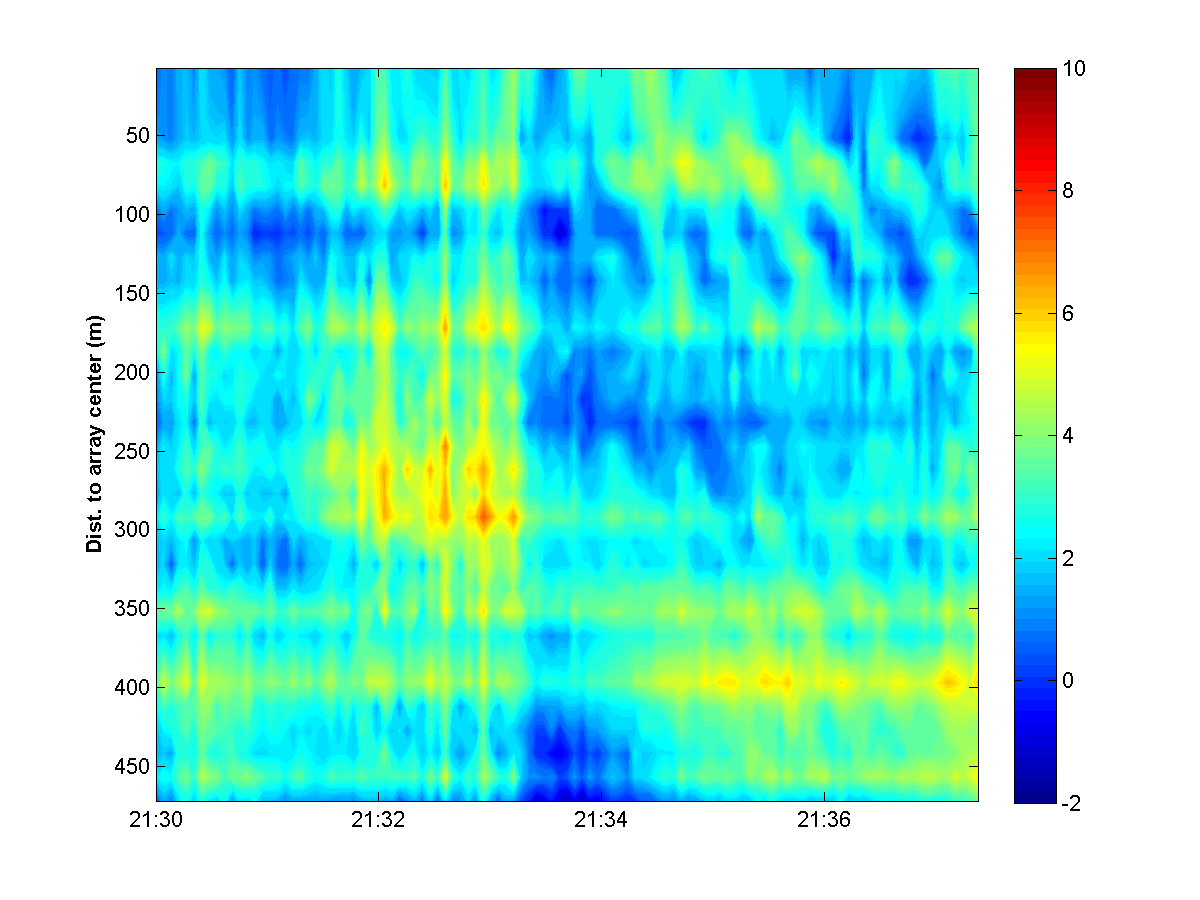
\includegraphics[width=0.5\textwidth,height=0.2\textwidth]{0817_2130_hla.png}\\
%  \end{tabular}
%  \caption{Received signal on Shark VLA (top), HLA (bottom) and signal intensity (middle) from Aug.17 21:30GMT to 21:37GMT }\label{fig:a2130}
%\end{figure}
%
%\begin{figure}[H]
%  \centering
%  \begin{tabular}{cc}
%  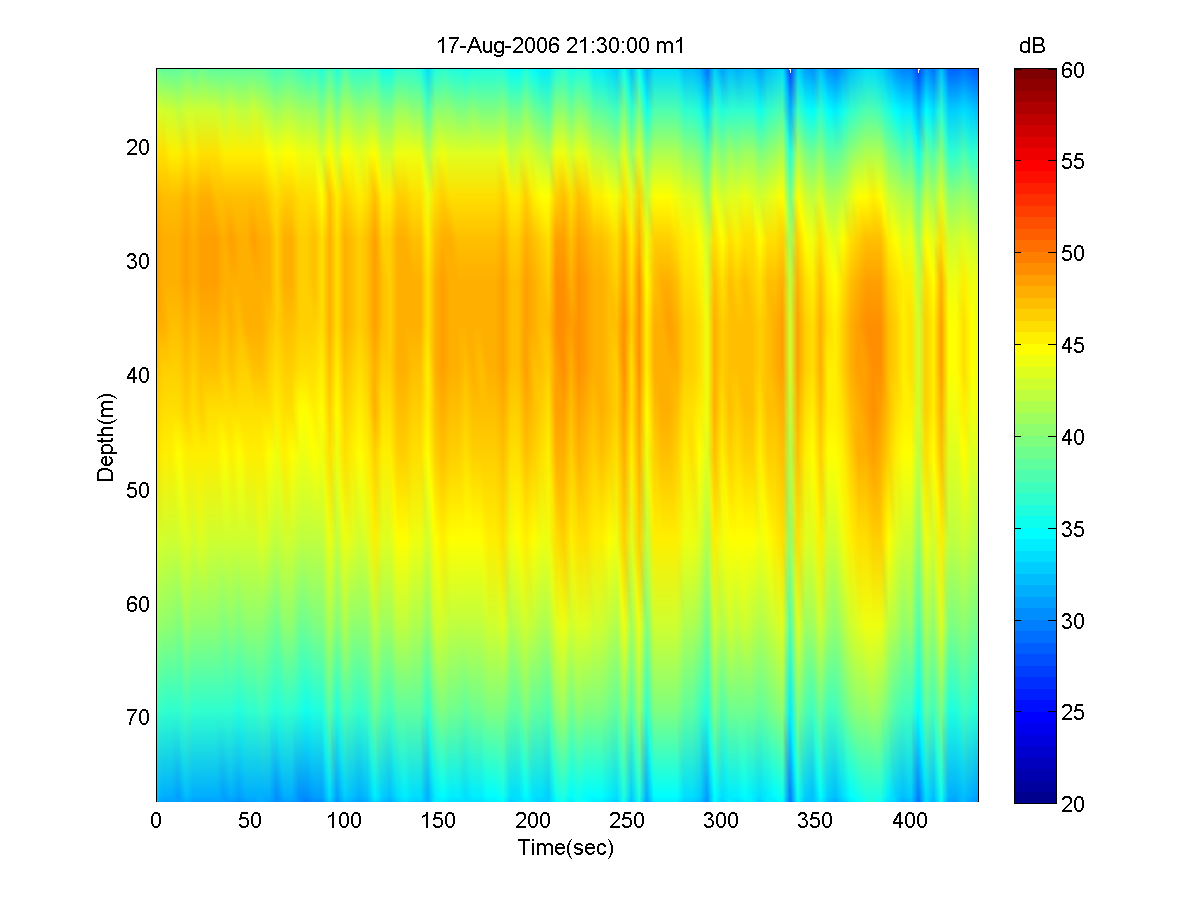
\includegraphics[width=0.5\textwidth,height=0.2\textwidth]{nrl_200608172130_m1.png}
%  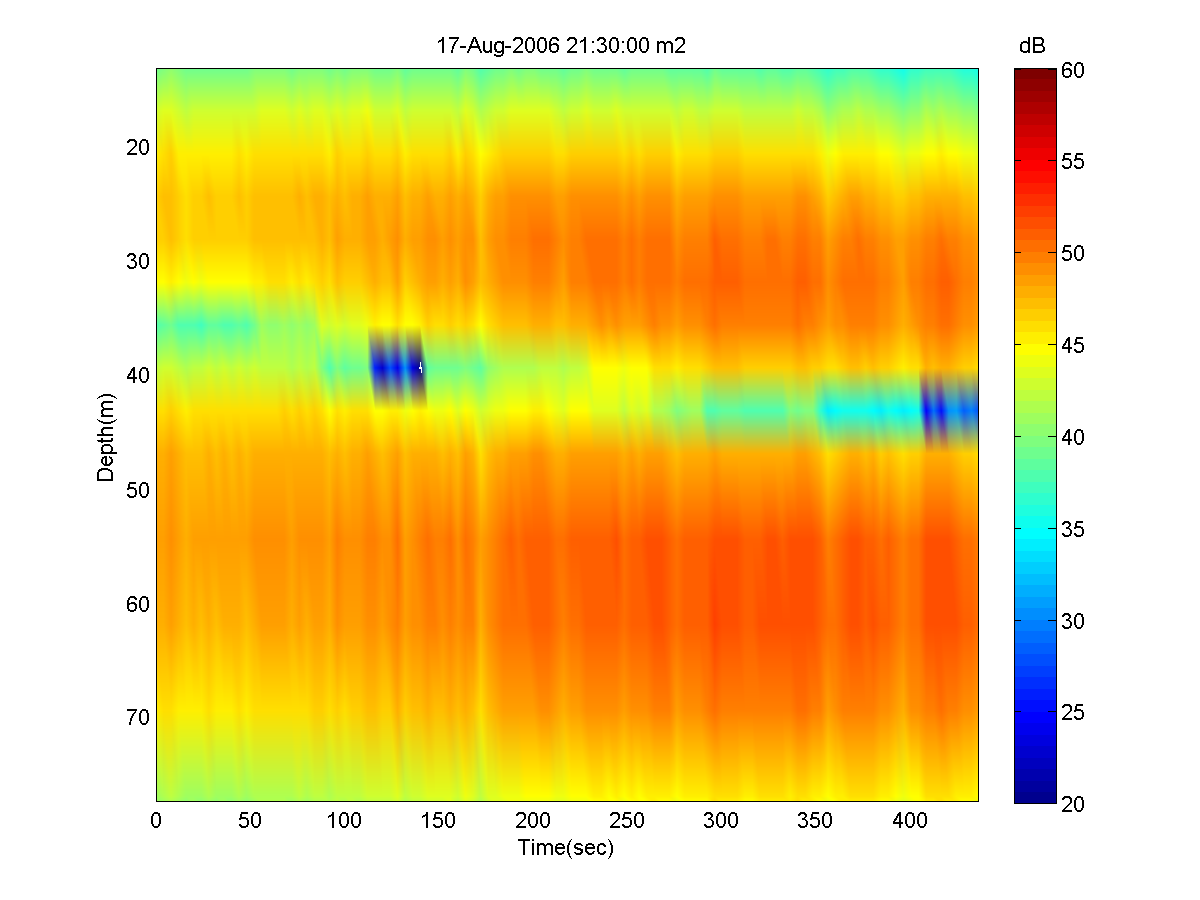
\includegraphics[width=0.5\textwidth,height=0.2\textwidth]{nrl_200608172130_m2.png}\\
%  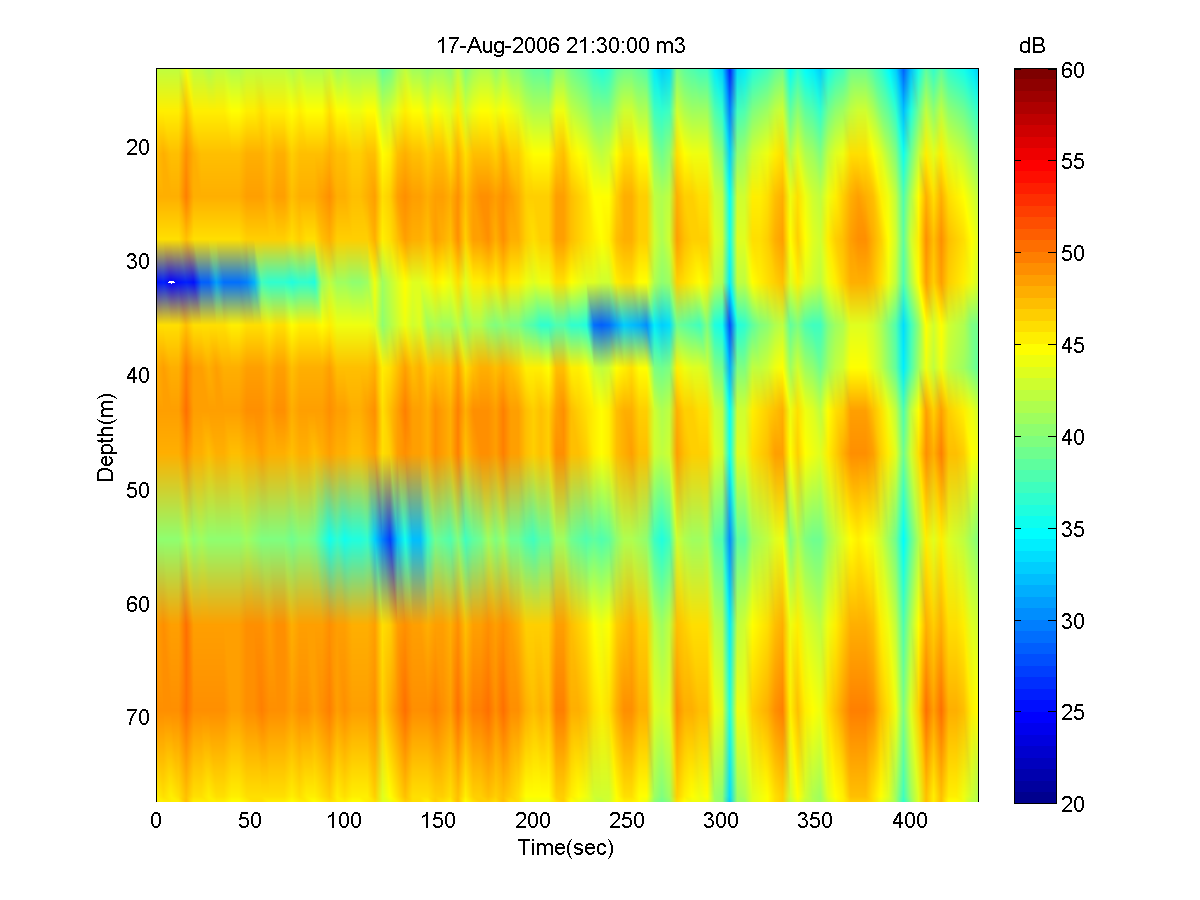
\includegraphics[width=0.5\textwidth,height=0.2\textwidth]{nrl_200608172130_m3.png}
%  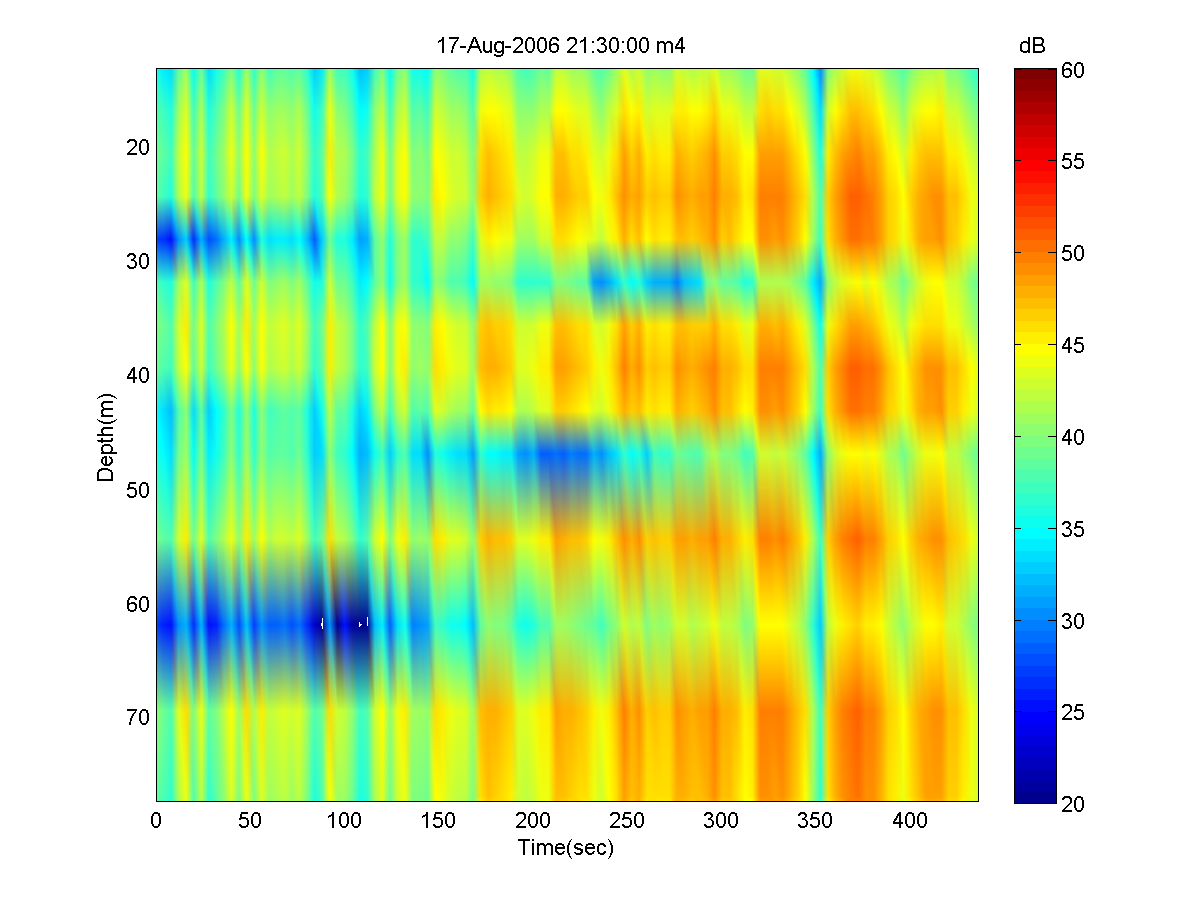
\includegraphics[width=0.5\textwidth,height=0.2\textwidth]{nrl_200608172130_m4.png}\\
%  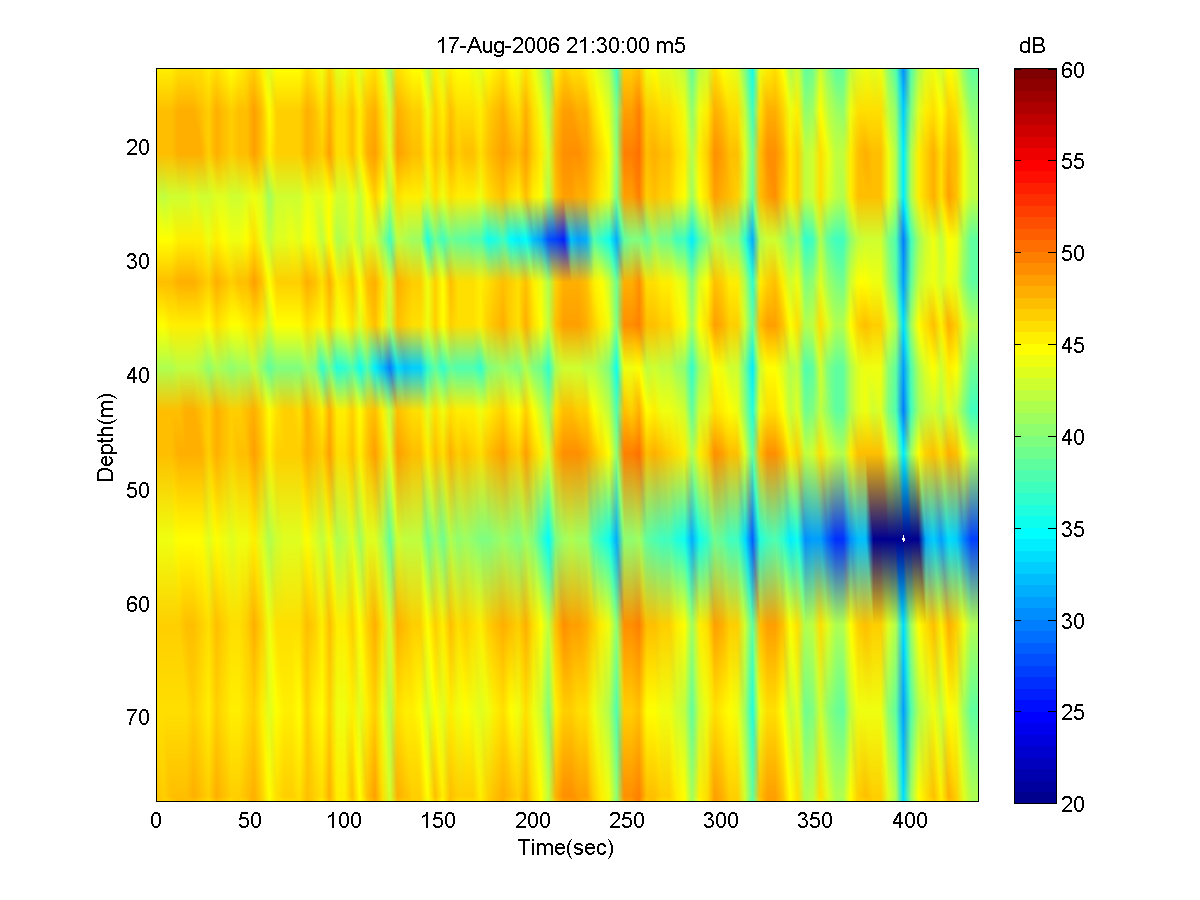
\includegraphics[width=0.5\textwidth,height=0.2\textwidth]{nrl_200608172130_m5.png}
%  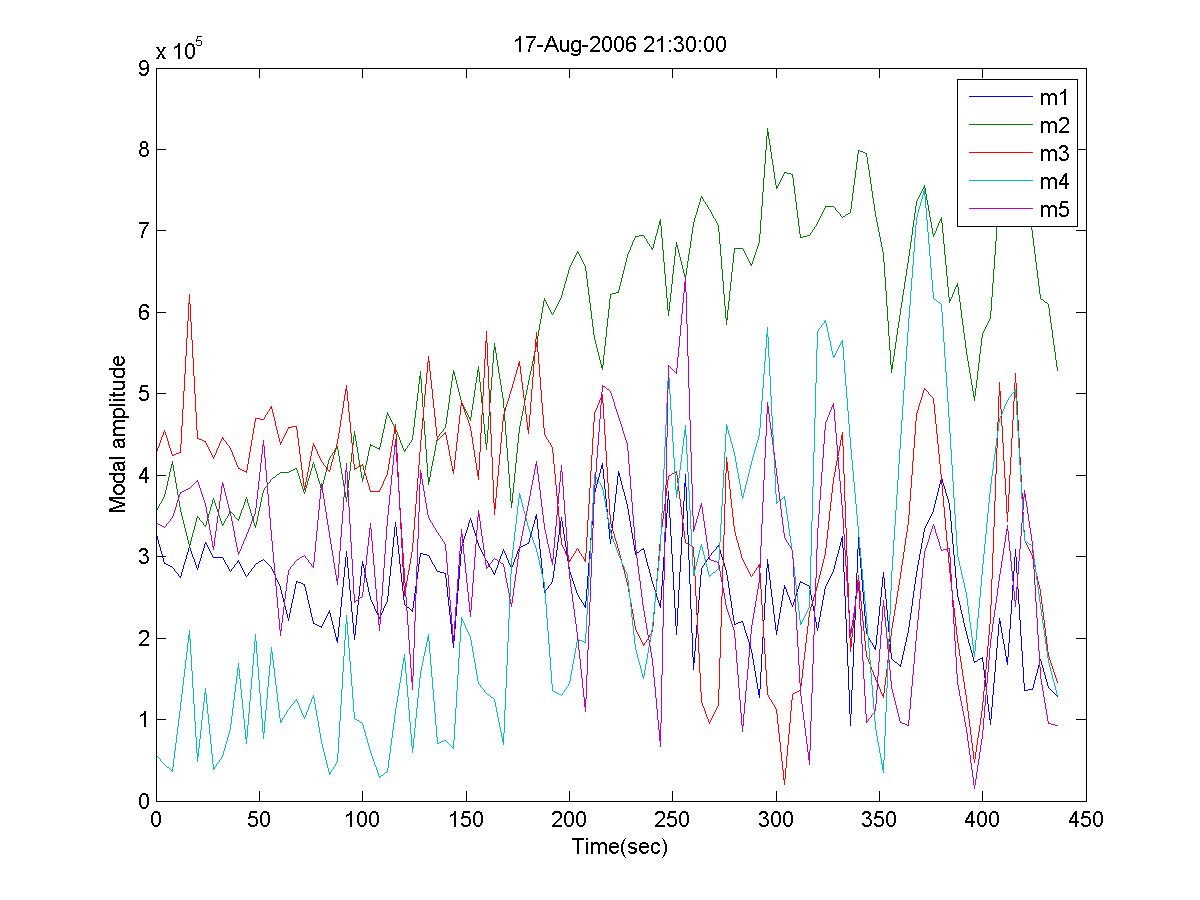
\includegraphics[width=0.5\textwidth,height=0.2\textwidth]{nrl_ma_200608172130.png}\\
%  \end{tabular}
%  \caption{Modal decomposition and amplitude of the signal received on Shark VLA from Aug.17 21:30GMT to 21:37GMT }\label{fig:m2130}
%\end{figure}

%\begin{figure}
 % \centering
  %\begin{tabular}{lrr}
  %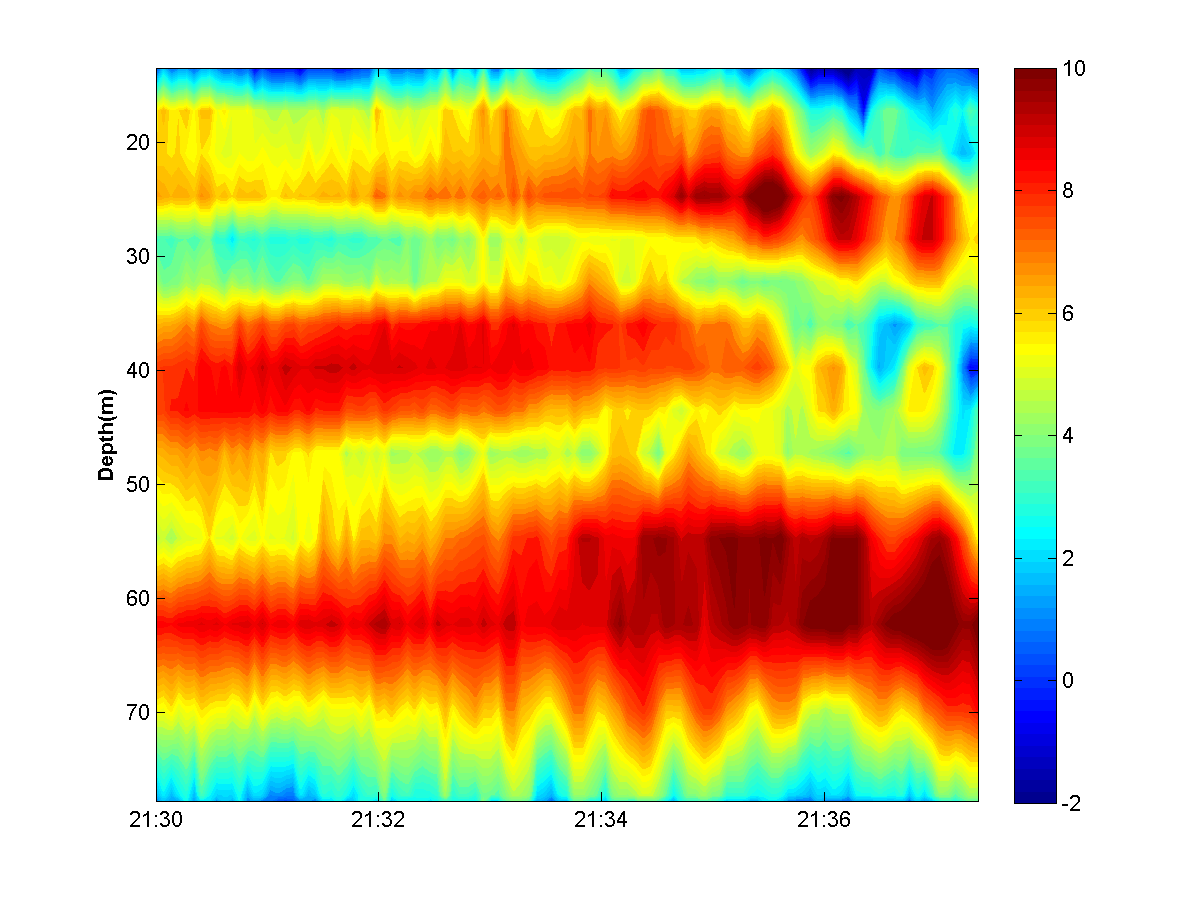
\includegraphics[width=0.3\textwidth,height=0.1\textwidth]{0817_2130_vla.png}
  %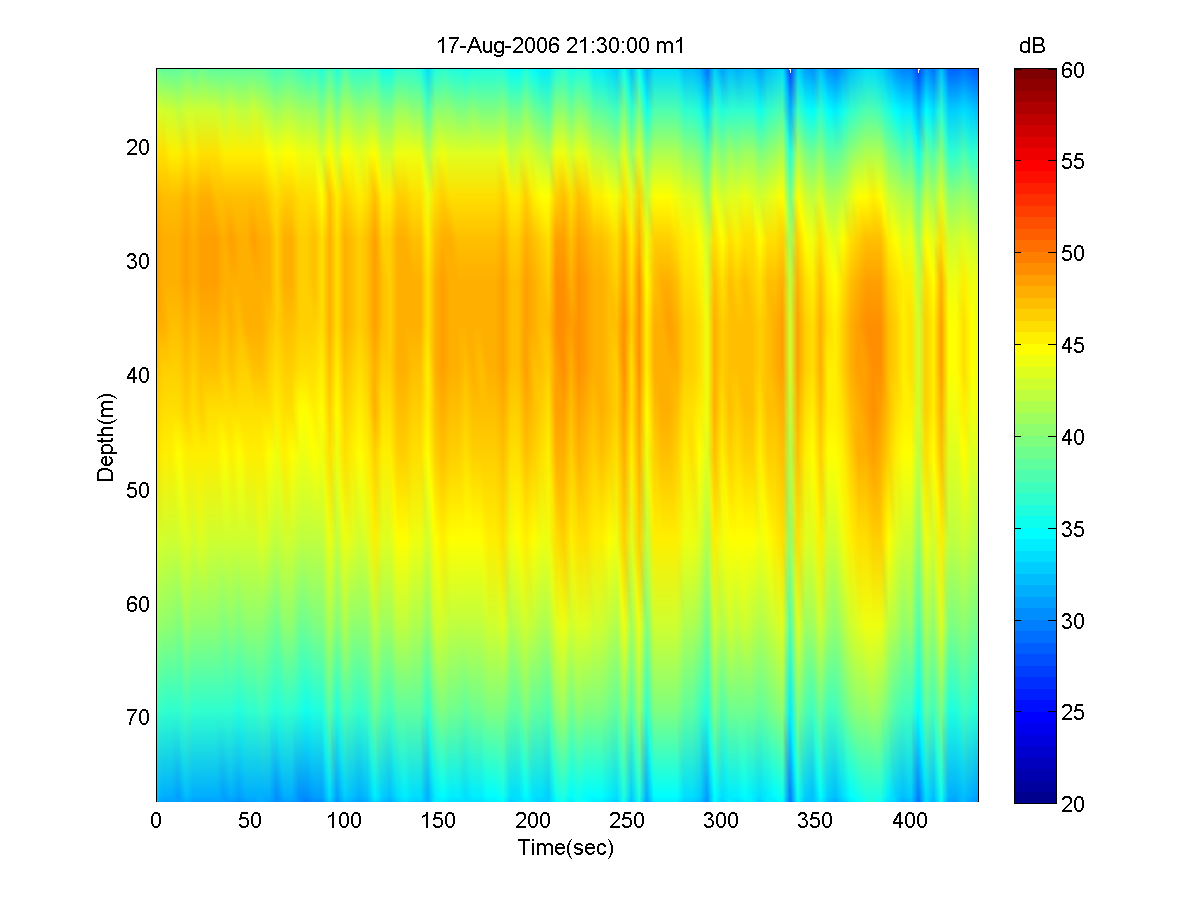
\includegraphics[width=0.3\textwidth,height=0.1\textwidth]{nrl_200608172130_m1.png}
  %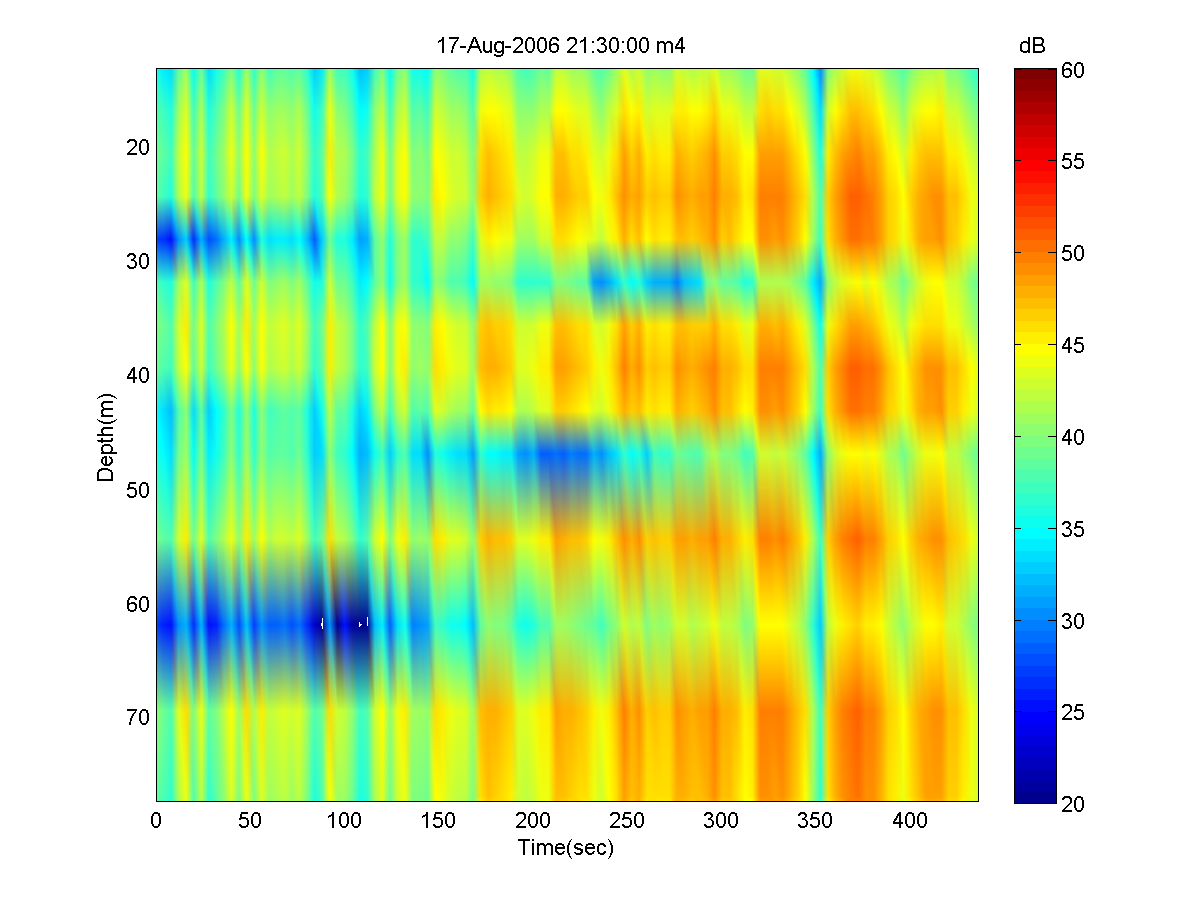
\includegraphics[width=0.3\textwidth,height=0.1\textwidth]{nrl_200608172130_m4.png}\\
  %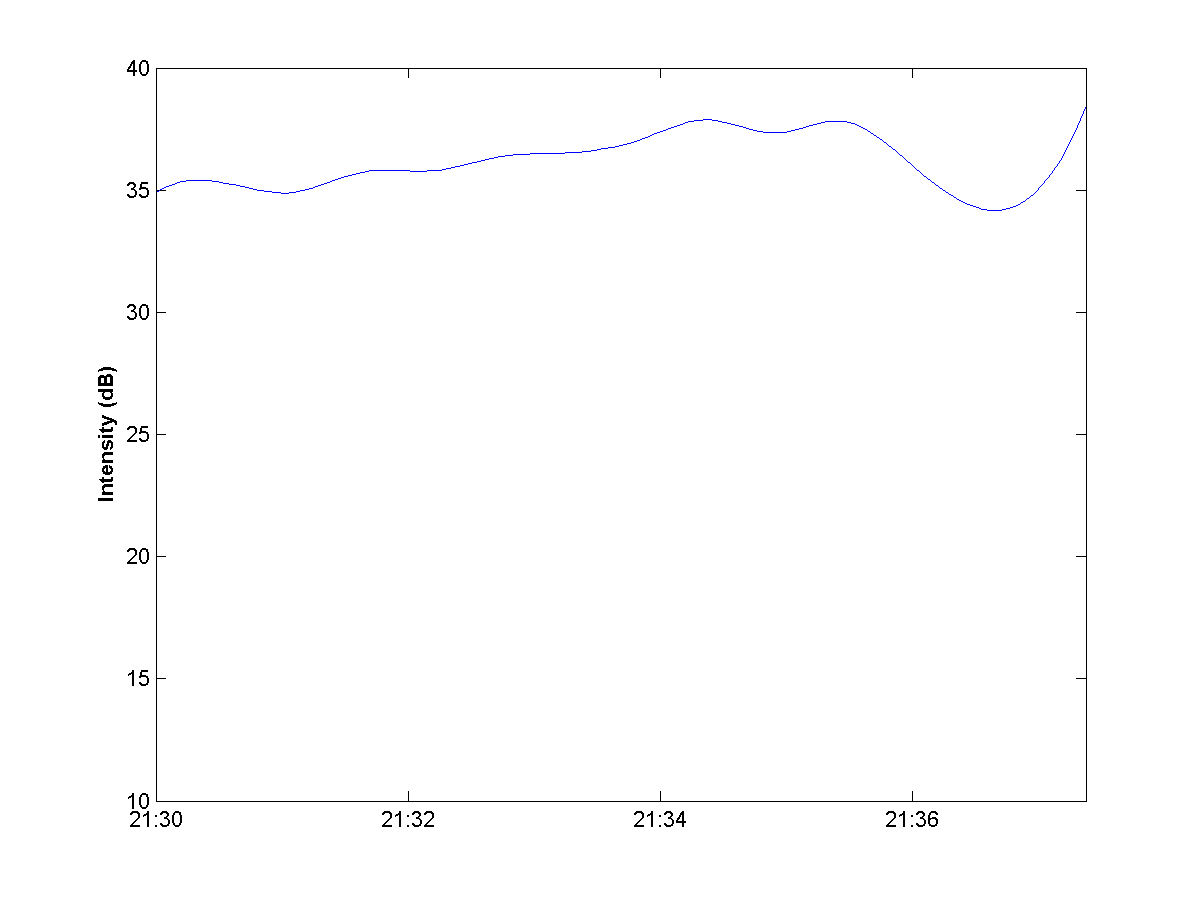
\includegraphics[width=0.3\textwidth,height=0.1\textwidth]{0817_2130_eng.png}
  %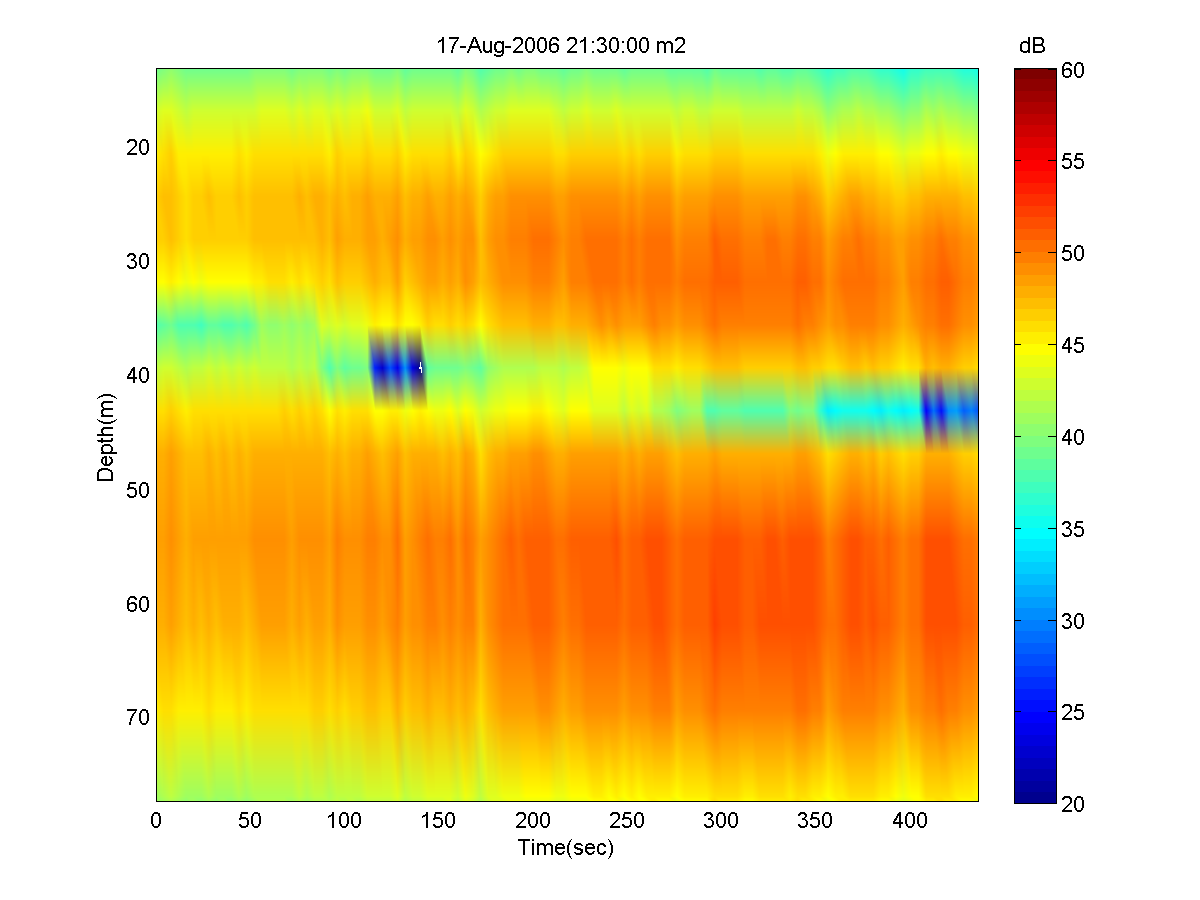
\includegraphics[width=0.3\textwidth,height=0.1\textwidth]{nrl_200608172130_m2.png}
  %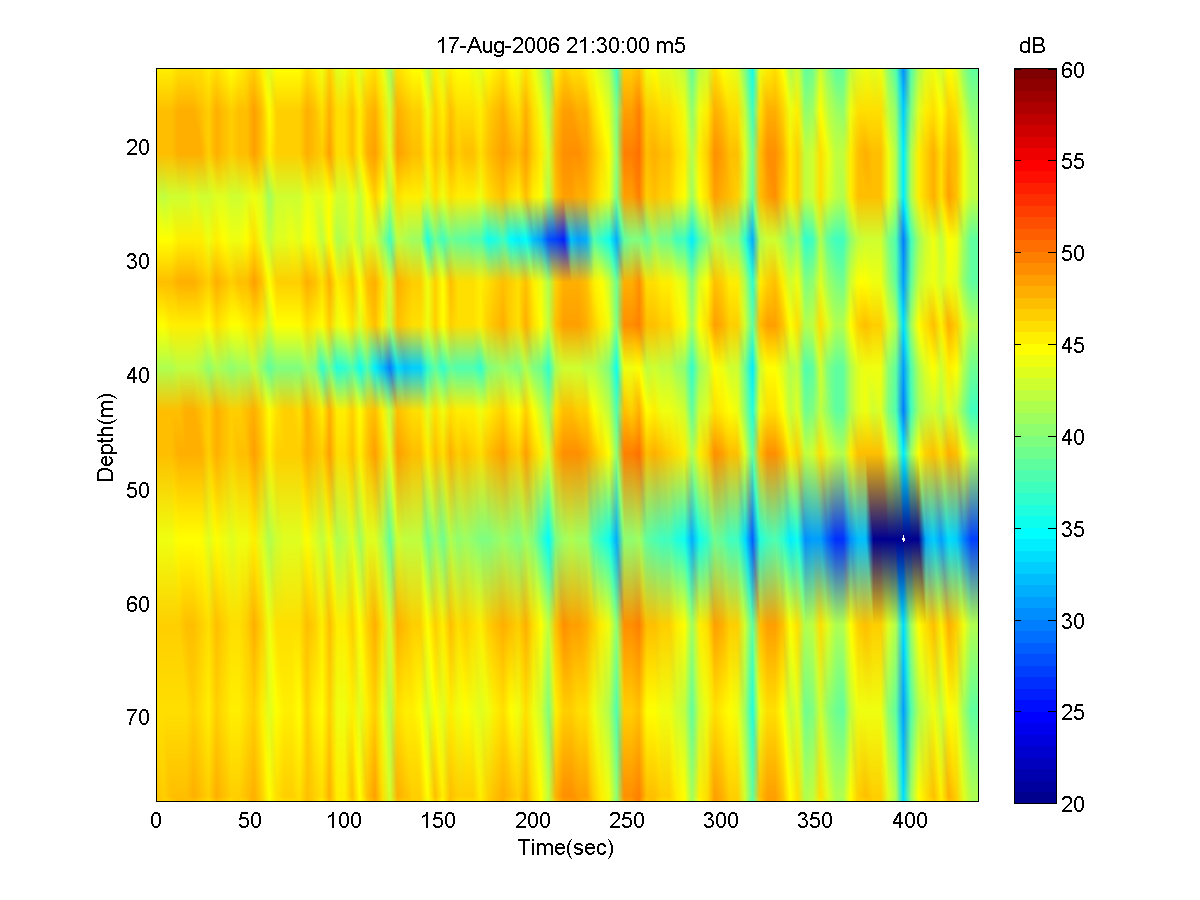
\includegraphics[width=0.3\textwidth,height=0.1\textwidth]{nrl_200608172130_m5.png}\\
  %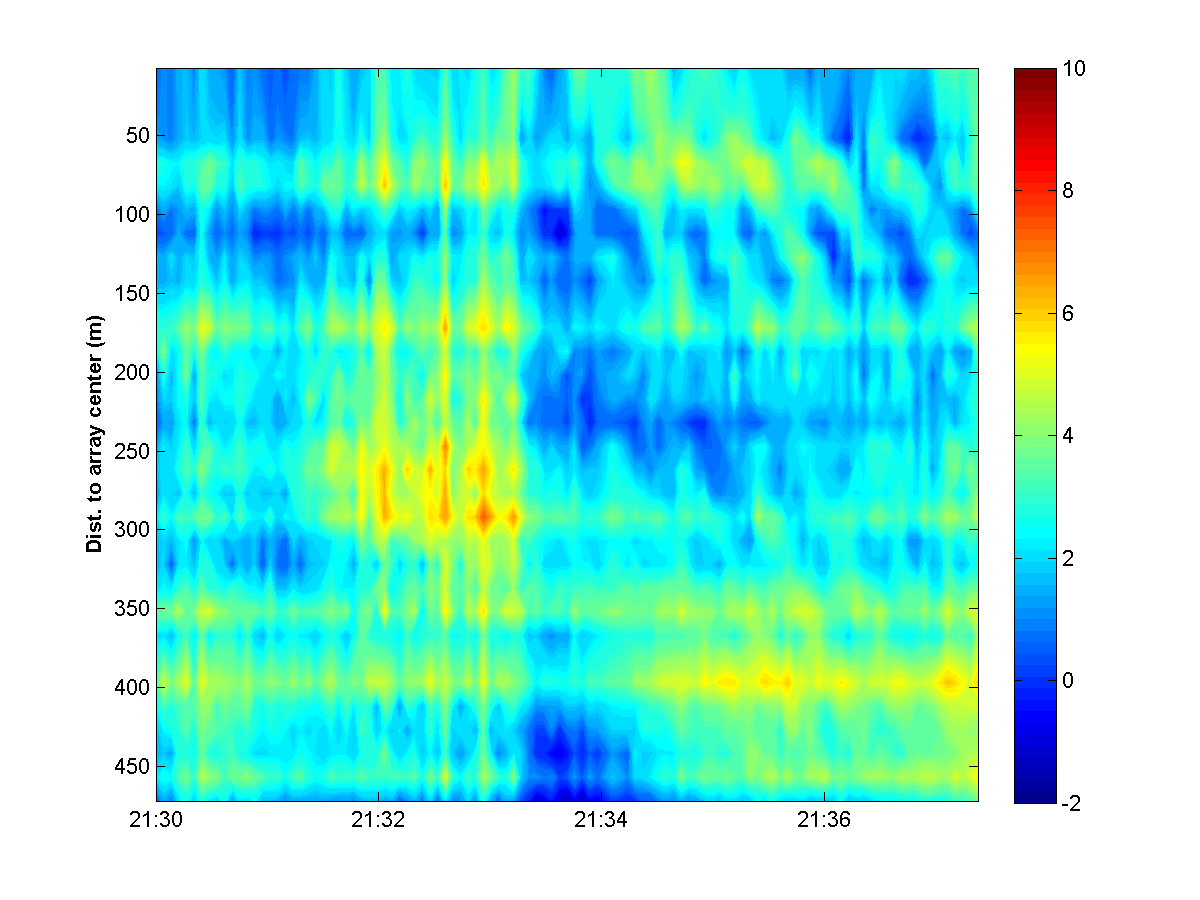
\includegraphics[width=0.3\textwidth,height=0.1\textwidth]{0817_2130_hla.png}
  %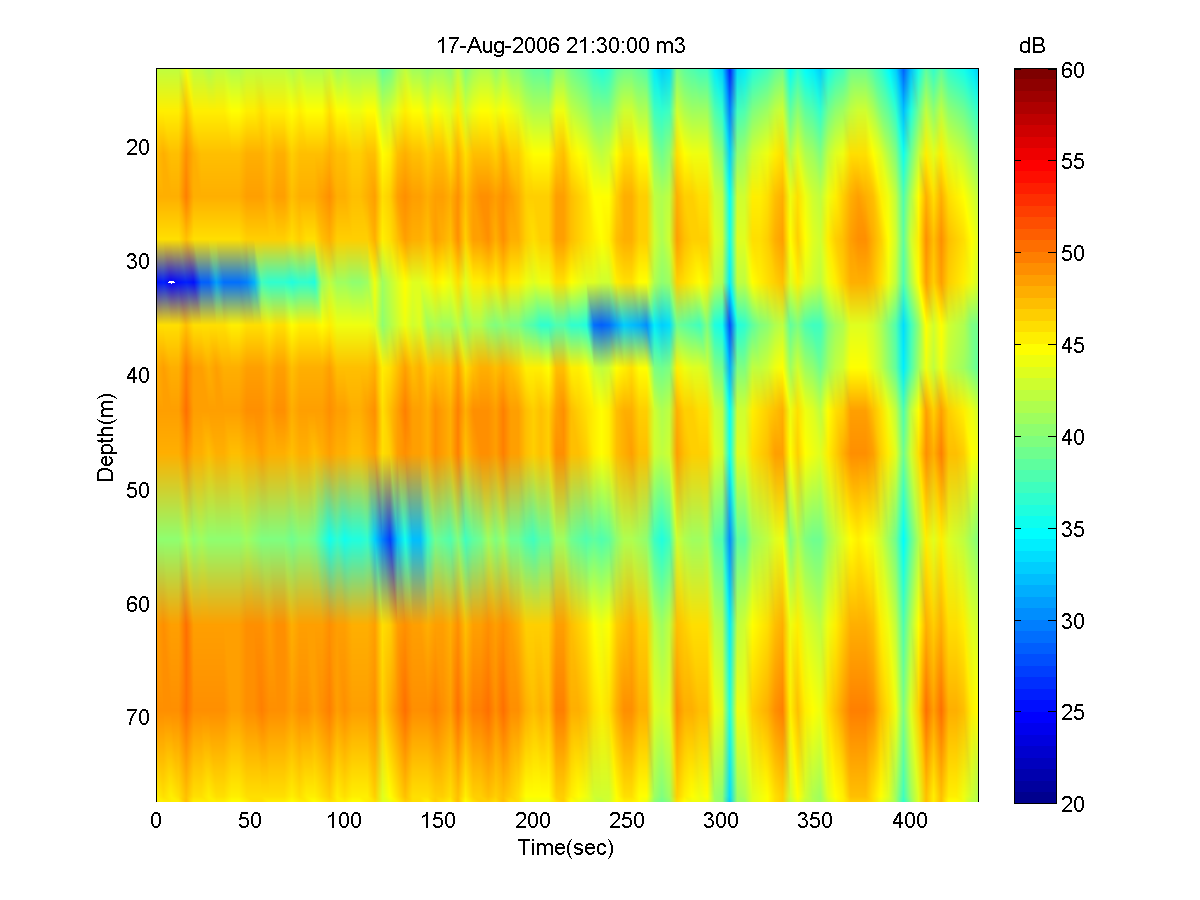
\includegraphics[width=0.3\textwidth,height=0.1\textwidth]{nrl_200608172130_m3.png}
  %\includegraphics[width=0.3\textwidth,height=0.1\textwidth]{nrl_ma_200608172130.png}\\
  %\end{tabular}
  %\caption{Received signal on Shark array from Aug.17 21:30GMT to 21:37GMT. Left column, from top to bottom: signal on VLA, VLA signal intensity, signal on HLA; middle column: mode 1-3; right column: mode 4, 5, and modal amplitudes.}\label{fig:m2130}
%\end{figure}
\subsection{Phase III: 22:00-22:07GMT, 22:30-22:37GMT, 23:00-23:07GMT \& 23:30-23:37GMT}
Phase III is when the acoustic signal propagates through the body of the IW packet. The position of the source and receiver in internal waves can cause fluctuations (>6dB) in the received signal by mechanisms like refraction, focusing and defocusing depending on the relative positions of the source and receiver in the internal waves. At 22:00GMT,  the source is about three kilometers from the leading wave front, but the Shark VlA is at the trough between the second and the third waves, and about half of the acoustic track is directly interacting with the IW packet. 
%
%ISW occupies the most of the acoustic path. Slopes on the HLA show
%the strong effects of ISW on the acoustic propagation. On the VLA,
%the focusing induces the intensity fluctuation of 15dB. Modal
%decomposition shows mode 1 is the dominant play of the focusing with
%a sudden increase in amplitude.
%\begin{figure}[H]
 % \centering
  %\includegraphics[width=0.5\textwidth]{radar2200.png}
  %\caption{Radar image of ISW at 21:30GMT}\label{fig:r2200}
%\end{figure}
%\begin{figure}
 % \centering
  %\begin{tabular}{lrr}
  %\includegraphics[width=0.3\textwidth,height=0.1\textwidth]{0817_2200_vla.png}
  %\includegraphics[width=0.3\textwidth,height=0.1\textwidth]{nrl_200608172200_m1.png}
  %\includegraphics[width=0.3\textwidth,height=0.1\textwidth]{nrl_200608172200_m4.png}\\
  %\includegraphics[width=0.3\textwidth,height=0.1\textwidth]{0817_2200_eng.png}
  %\includegraphics[width=0.3\textwidth,height=0.1\textwidth]{nrl_200608172200_m2.png}
  %\includegraphics[width=0.3\textwidth,height=0.1\textwidth]{nrl_200608172200_m5.png}\\
  %\includegraphics[width=0.3\textwidth,height=0.1\textwidth]{0817_2200_hla.png}
  %\includegraphics[width=0.3\textwidth,height=0.1\textwidth]{nrl_200608172200_m3.png}
  %\includegraphics[width=0.3\textwidth,height=0.1\textwidth]{nrl_ma_200608172200.png}\\
  %\end{tabular}
  %\caption{Received signal on Shark array from Aug.17 20:30GMT to 20:37GMT. Left column, from top to bottom: signal on VLA, VLA signal intensity, signal on HLA; middle column: mode 1-3; right column: mode 4, 5, and modal amplitudes.}\label{fig:m2200}
%\end{figure}
\subsection{Phase IV: after 23:30GMT}
This is the afterward phase when the entire IW packet has well passed acoustic track and has no noticeable acoustical impact. 
The acoustic path is at the middle of the ISW package, where the
wavelength is shorter than the leading fronts. Two focusing events
are observed with 15dB variations on total intensity. Mode 1 and 2
show more fluctuation than mode 3, 4 and 5. On HLA, regular slopes
are shown, sometimes not consistent with the signals on VLA.
%\begin{figure}[H]
 % \centering
  %\includegraphics[width=0.5\textwidth]{radar2230.png}
  %\caption{Radar image of ISW at 21:30GMT}\label{fig:r2230}
%\end{figure}
%\begin{figure}
  %\centering
  %\begin{tabular}{lrr}
  %\includegraphics[width=0.3\textwidth,height=0.1\textwidth]{0817_2230_vla.png}
  %\includegraphics[width=0.3\textwidth,height=0.1\textwidth]{nrl_200608172230_m1.png}
  %\includegraphics[width=0.3\textwidth,height=0.1\textwidth]{nrl_200608172230_m4.png}\\
  %\includegraphics[width=0.3\textwidth,height=0.1\textwidth]{0817_2230_eng.png}
  %\includegraphics[width=0.3\textwidth,height=0.1\textwidth]{nrl_200608172230_m2.png}
  %\includegraphics[width=0.3\textwidth,height=0.1\textwidth]{nrl_200608172230_m5.png}\\
  %\includegraphics[width=0.3\textwidth,height=0.1\textwidth]{0817_2230_hla.png}
  %\includegraphics[width=0.3\textwidth,height=0.1\textwidth]{nrl_200608172230_m3.png}
  %\includegraphics[width=0.3\textwidth,height=0.1\textwidth]{nrl_ma_200608172230.png}\\
  %\end{tabular}
  %\caption{Received signal on Shark array from Aug.17 22:30GMT to 22:37GMT. Left column, from top to bottom: signal on VLA, VLA signal intensity, signal on HLA; middle column: mode 1-3; right column: mode 4, 5, and modal amplitudes.}\label{fig:m2230}
%\end{figure}
\subsection{23:00GMT-23:07GMT}
The acoustic path now is at the coverage of R/V Sharp's radar, and
escapes from R/V Oceanouse's radar. From the temperature plot, the
acoustic path is still affected by the ISW package. Tow focusing
events are shown with about 15dB fluctuation.
%\begin{figure}[H]
 % \centering
%  \includegraphics[width=0.5\textwidth]{radar2300.png}
 % \caption{Radar image of ISW at 21:30GMT}\label{fig:r2300}
%\end{figure}
%\begin{figure}
 % \centering
  %\begin{tabular}{lrr}
  %\includegraphics[width=0.3\textwidth,height=0.1\textwidth]{0817_2300_vla.png}
  %\includegraphics[width=0.3\textwidth,height=0.1\textwidth]{nrl_200608172300_m1.png}
  %\includegraphics[width=0.3\textwidth,height=0.1\textwidth]{nrl_200608172300_m4.png}\\
  %\includegraphics[width=0.3\textwidth,height=0.1\textwidth]{0817_2300_eng.png}
  %\includegraphics[width=0.3\textwidth,height=0.1\textwidth]{nrl_200608172300_m2.png}
  %\includegraphics[width=0.3\textwidth,height=0.1\textwidth]{nrl_200608172300_m5.png}\\
  %\includegraphics[width=0.3\textwidth,height=0.1\textwidth]{0817_2300_hla.png}
  %\includegraphics[width=0.3\textwidth,height=0.1\textwidth]{nrl_200608172300_m3.png}
  %\includegraphics[width=0.3\textwidth,height=0.1\textwidth]{nrl_ma_200608172300.png}\\
  %\end{tabular}
  %\caption{Received signal on Shark array from Aug.17 23:00GMT to 23:07GMT. Left column, from top to bottom: signal on VLA, VLA signal intensity, signal on HLA; middle column: mode 1-3; right column: mode 4, 5, and modal amplitudes.}\label{fig:m2300}
%\end{figure}
\subsection{23:30GMT-23:37GMT}
No radar image, but the temperature plots shows the acoustic path is
still under the influence of ISW. Tow focusing events are recorded
on HLA with fluctuation about 15dB.
%\begin{figure}[H]
 % \centering
 % \includegraphics[width=0.5\textwidth]{radar2330.png}
  %\caption{Radar image of ISW at 21:30GMT}\label{fig:r2330}
%\end{figure}
%\begin{figure}
  %\centering
  %\begin{tabular}{lrr}
  %\includegraphics[width=0.3\textwidth,height=0.1\textwidth]{0817_2330_vla.png}
  %\includegraphics[width=0.3\textwidth,height=0.1\textwidth]{nrl_200608172330_m1.png}
  %\includegraphics[width=0.3\textwidth,height=0.1\textwidth]{nrl_200608172330_m4.png}\\
  %\includegraphics[width=0.3\textwidth,height=0.1\textwidth]{0817_2330_eng.png}
  %\includegraphics[width=0.3\textwidth,height=0.1\textwidth]{nrl_200608172330_m2.png}
  %\includegraphics[width=0.3\textwidth,height=0.1\textwidth]{nrl_200608172330_m5.png}\\
  %\includegraphics[width=0.3\textwidth,height=0.1\textwidth]{0817_2330_hla.png}
  %\includegraphics[width=0.3\textwidth,height=0.1\textwidth]{nrl_200608172330_m3.png}
  %\includegraphics[width=0.3\textwidth,height=0.1\textwidth]{nrl_ma_200608172330.png}\\
  %\end{tabular}
  %\caption{Received signal on Shark array from Aug.17 23:30GMT to 23:37GMT. Left column, from top to bottom: signal on VLA, VLA signal intensity, signal on HLA; middle column: mode 1-3; right column: mode 4, 5, and modal amplitudes.}\label{fig:m2330}
%\end{figure}


%%------------------------------------------------%%
